\documentclass[12 pt]{article}
\usepackage{graphicx}  % Required for inserting images
\usepackage{listings}
\usepackage[colorlinks=true, urlcolor=blue]{hyperref}
\usepackage[style=numeric,backend=biber,hyperref]{biblatex}
\usepackage{float}
\addbibresource{references.bib}

\usepackage[a4paper,margin= 1 in]{geometry}
\usepackage{enumerate}

\usepackage{xcolor} % Required for custom colors

% Define custom colors
\definecolor{commentColor}{rgb}{0.5,0.5,0.5} % Grey for comments
\definecolor{keywordColor}{rgb}{0,0,1}       % Blue for keywords
\definecolor{stringColor}{rgb}{0.58,0,0.82}  % Purple for strings

% Define custom Bash script style
\lstdefinestyle{BashStyle}{
    language=bash,
    basicstyle=\ttfamily\small, % Monospaced font
    breakatwhitespace=false,         
    breaklines=true,                 
    captionpos=b,                    
    keepspaces=true,                 
    showspaces=false,                
    showstringspaces=false,
    showtabs=false,                  
    tabsize=2
}

% Apply the custom style
\lstset{style=BashStyle}

% To write a custom bash script
% \begin{lstlisting}[language=bash]
% $ ls -l
% total 32
% -rw-r--r-- 1 user user  237 Mar  8 10:00 file1.txt
% -rw-r--r-- 1 user user 1566 Mar  8 09:59 file2.txt
% drwxr-xr-x 2 user user 4096 Mar  8 09:59 images
% \end{lstlisting}

% \title{1905097 1905105 Gobuster report}
% \author{Shahriar Raj, Abrar Mahmud}
% \date{March 2024}

\begin{document}

\begin{titlepage}
    \centering
    {\scshape\Large CSE 406 Project Report\par}
    \vspace{1.5cm}
    {\huge\bfseries GOBUSTER : A Content Discovery Tool\par}
    \vspace{2cm}
    {\Large\itshape Report Prepared by:\par}
    \vspace{0.25cm}
    {\scshape\Large Abrar Mahmud - 1905097\par} 
    {\scshape\Large Shahriar Raj - 1905105\par} 
    \vspace{2cm}
    {\Large\itshape Supervised by:\par}
    \vspace{0.25cm}
    {\scshape\Large A.K.M Mehedi Hasan\par}
    \vspace{2cm}
    {\scshape\LARGE Department of CSE, BUET \par}
    \vfill
    % Bottom of the page
\end{titlepage}

\newpage
\tableofcontents
\newpage

\section{Introduction}
Gobuster is a powerful, open-source tool designed to enumerate files and directories on web/application servers. It is written in Go, making it capable of doing high-performance work. Gobuster is commonly used by cybersecurity professionals, including penetration testers and ethical hackers, to discover hidden resources within web servers and DNS structures that are not typically visible or linked from the main pages of a website. 
\\ \\
The tool operates by using wordlists that contain numerous filenames, directory names, or subdomains. These wordlists are used as the basis to systematically check for the existence of resources on the target server or domain. Gobuster can identify potentially unsecured files, directories, and subdomains that might expose sensitive information or reveal insights about the backend structure of the web application, thus highlighting areas that may require further investigation or immediate security measures. The tool is mainly Linux-based.\\
\subsection{\underline{Key Features of Gobuster}}
\begin{itemize}
    \item \textbf{Directory/File Enumeration:} Quickly identifies hidden or unlisted directories and files on web servers by brute-forcing URIs using wordlists.
    \item \textbf{DNS Subdomain Enumeration:} Discovers subdomains by brute-forcing domain name systems, helping to map out a target's DNS structure.
    \item \textbf{Virtual Host Scanning:} Can identify virtual hosts configured on web servers.
    \item \textbf{Support for Various Protocols:} Works with HTTP, HTTPS, and supports other schemes by integrating with proxy servers.
    \item \textbf{Customizable:} Supports various flags and configurations to customize scans, including setting custom headers, using cookies, and ignoring SSL/TLS certificate warnings.
    \item \textbf{Concurrent Processing:} Utilizes the Go language's powerful concurrency features to perform multiple requests or queries simultaneously, significantly speeding up the enumeration process.
    \item \textbf{Flexible:} Allows users to exclude certain response sizes, specify status codes to find or ignore, and even resume interrupted scans.
\end{itemize} 

\subsection{Why use Gobuster?}
\begin{itemize}
\item It is free and OpenSource
\item It is fast and easy to run
\item Can be used with customized wordlists
\item Supports various protocols beyond HTTP/HTTPS like FTP
\end{itemize} 
Gobuster is popular in the cybersecurity community for its simplicity, speed, and effectiveness. It's an essential tool in the vulnerability assessment and penetration testing processes, aiding in the early stages of assessment by providing insights into possible points of entry and areas requiring deeper security analysis. Whether used for educational purposes, ethical hacking, or professional cybersecurity assessments, Gobuster serves as a critical component in the toolkit of modern security practitioners, emphasizing the importance of proactive security measures and thorough digital infrastructure examination.
\section{Installation}
\textbf{Pre Requirements for Gobuster Installation: }\\
\begin{itemize}
\item Linux (Preferably Kali Linux) 
\item go (atleast version 1.16)
\end{itemize}
\textbf{\underline{Installing go:} }
\begin{lstlisting}[language=bash]
sudo apt update
sudo apt install golang-go
\end{lstlisting}
\textbf{\underline{Installing gobuster:} }
\begin{lstlisting}[language=bash]
sudo apt install gobuster
\end{lstlisting}
\section{Source Code Overview}
Gobuster is a content discovery tool written in \textbf{go} language. The source code link can be found in the following link: \cite{github}\\ \\
Each mode of operation is implemented in a different folder in gobuster. Short description of each part is given below:

\subsection{cli}
The cli directory is used for parsing the command line argument and showing output to the console or to a file. If we look at the file \textbf{gobuster.go} in the cli folder, we can find some goroutine functions.
\begin{itemize}
    \item \textbf{resultWorker:} It listens for results from \textbf{libgobuster.Gobuster} on a channel, formats the results into a string, and prints them to the console or to an output file.
    \item \textbf{errorWorker:} It listens for errors from \textbf{libgobuster.Gobuster} on a channel and prints the errors.
    \item \textbf{messageWorker:} It listens for log messages from \textbf{libgobuster.Gobuster} on a channel and prints the log messages based on their levels(debug, error and info).
    \item \textbf{progressWorker:} It uses a ticker to print the progress at regular intervals.
\end{itemize}  
\begin{figure}[H]
    \centering
    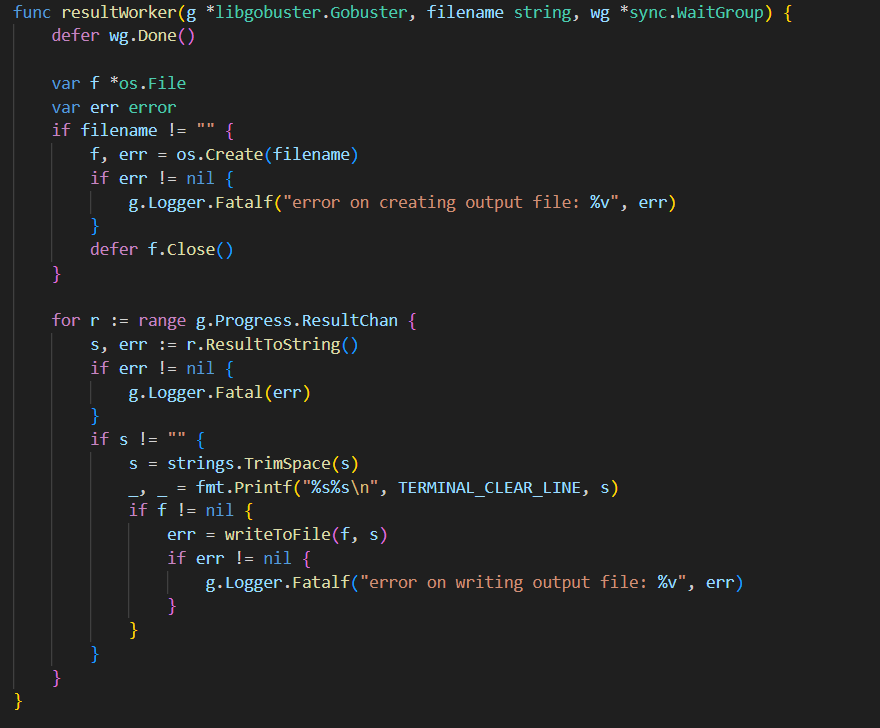
\includegraphics[width=0.4\textwidth]{resultWorker.png}
    \caption{resultWorker Function}
    \label{fig: resultWorker}
\end{figure}
\begin{figure}[H]
    \centering
    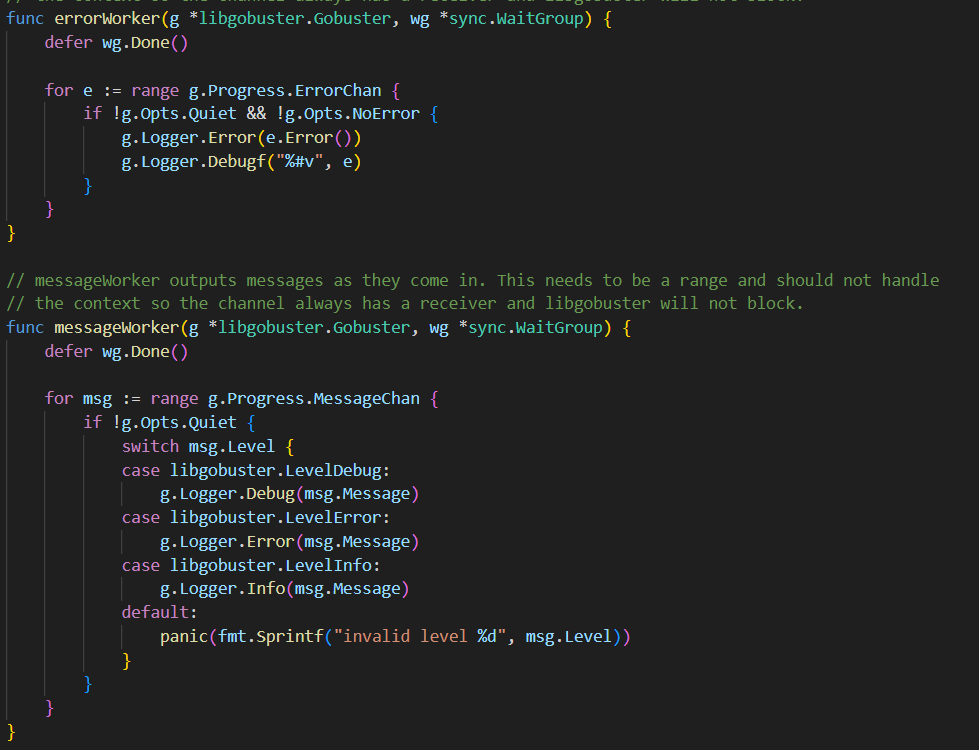
\includegraphics[width=0.4\textwidth]{errorWorker_messageWorker.png}
    \caption{errorWorker and messageWorker Function}
    \label{fig: errorWorker and messageWorker}
\end{figure}
\begin{figure}[H]
    \centering
    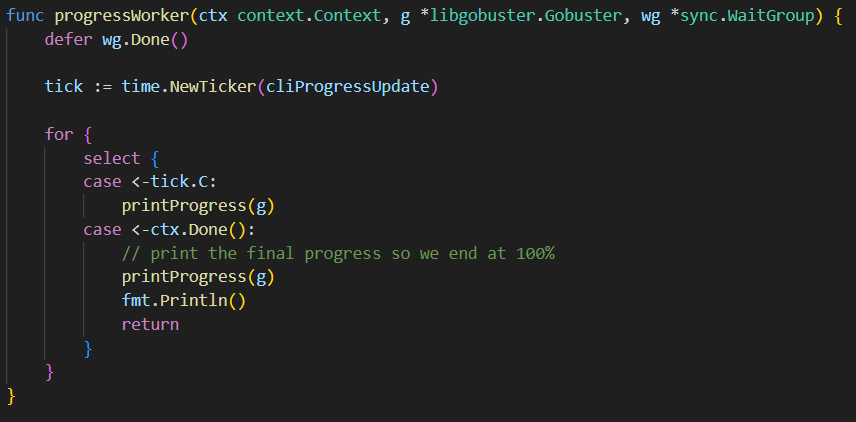
\includegraphics[width=0.4\textwidth]{progressWorker.png}
    \caption{progressWorker Function}
    \label{fig: progressWorker}
\end{figure}
The \textbf{Gobuster} function is the main entry point of the CLI. It sets up the environment, initializes \textbf{libgobuster.Gobuster}, and starts goroutines for workers. It first prints the Gobuster version and configuration details. Then it runs the Gobuster scan with the given context, waits for it to complete, and cleans up after.
\begin{figure}[H]
    \centering
    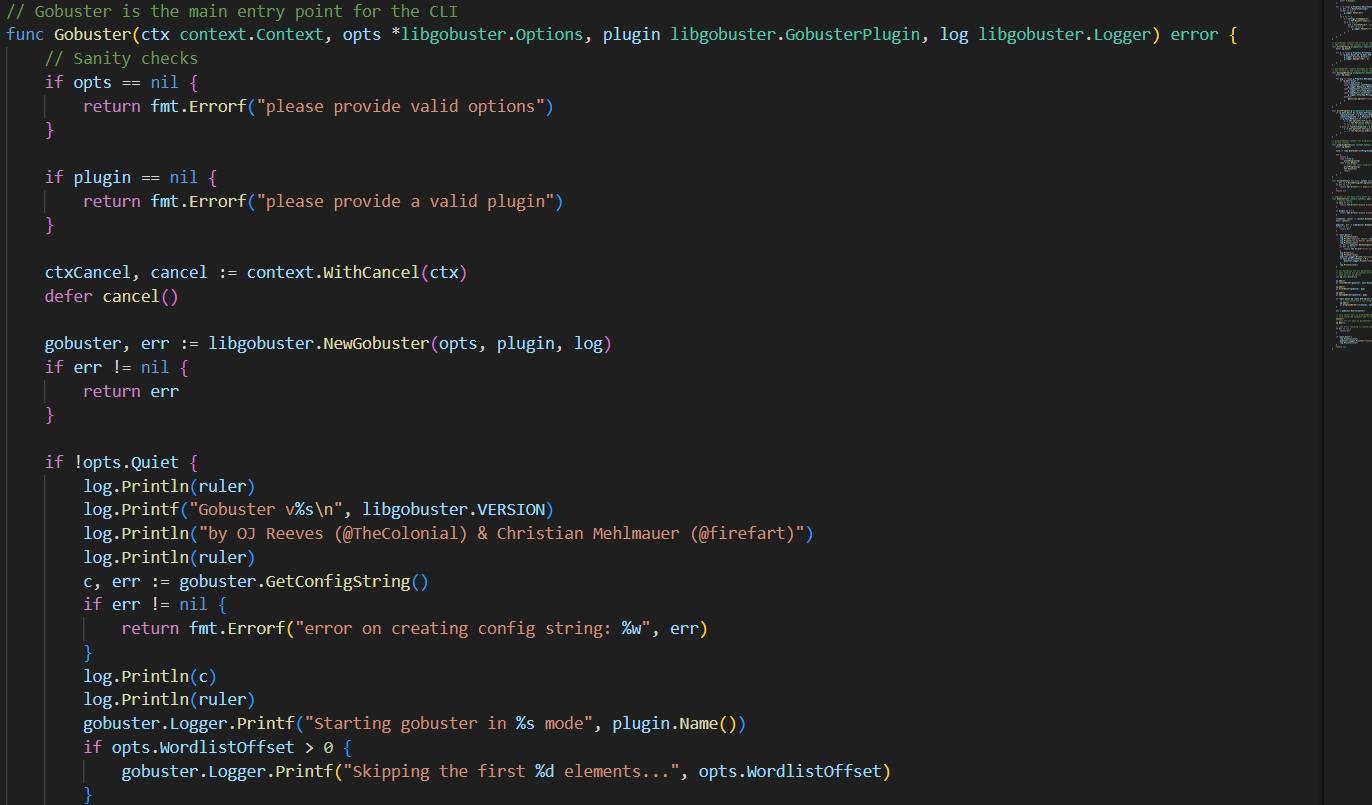
\includegraphics[width=0.4\textwidth]{Gobuster_cli.png}
    \caption{Gobuster Function}
    \label{fig: Gobuster cli}
\end{figure}
\subsection{libgobuster}
The libgobuster directory declares the basic interface of our gobuster object. We can see the basic interface of the gobuster object in the libgobuster.go file of the current folder.
\begin{figure}[H]
    \centering
    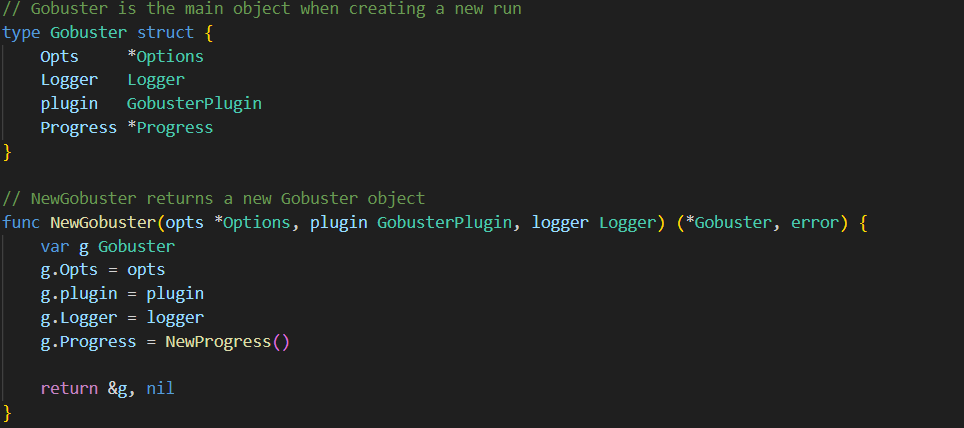
\includegraphics[width=0.4\textwidth]{Gobuster_struct.png}
    \caption{Structure of a Gobuster Object}
    \label{fig: Gobuster struct}
\end{figure}
The opts parameter defines the mode of operation and the related flags of that mode. Each mode of operation extends this struct to show their outputs.\\
\begin{figure}[H]
    \centering
    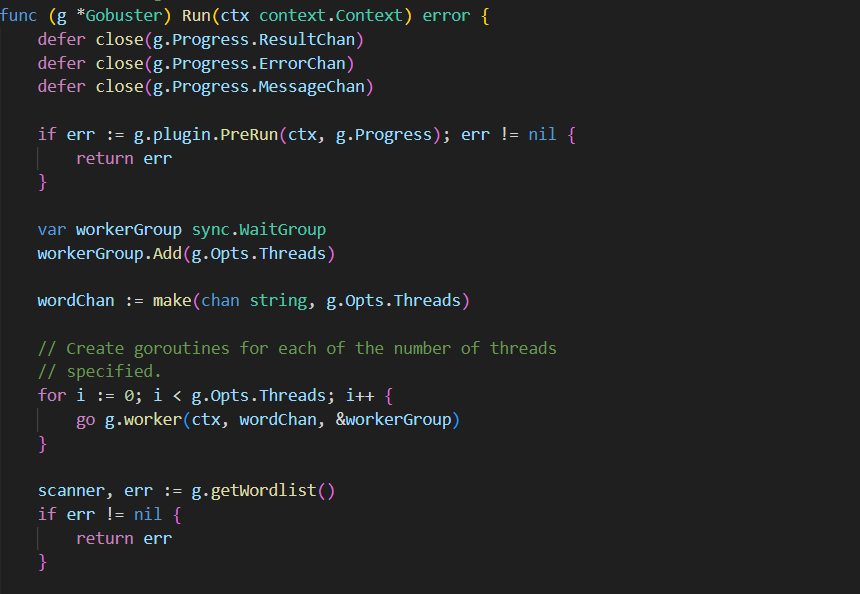
\includegraphics[width=0.4\textwidth]{Libgobuster_Run.png}
    \caption{Run function of a Gobuster Object}
    \label{fig: Libgobuster Run}
\end{figure} \\
The \textbf{Run} function creates a word channel, takes words as inputs and then uses the \textbf{worker} function. In the worker function, the \textbf{processWord} function does all mode specific operations. All modes implement this function differently.\\
\begin{figure}[H]
    \centering
    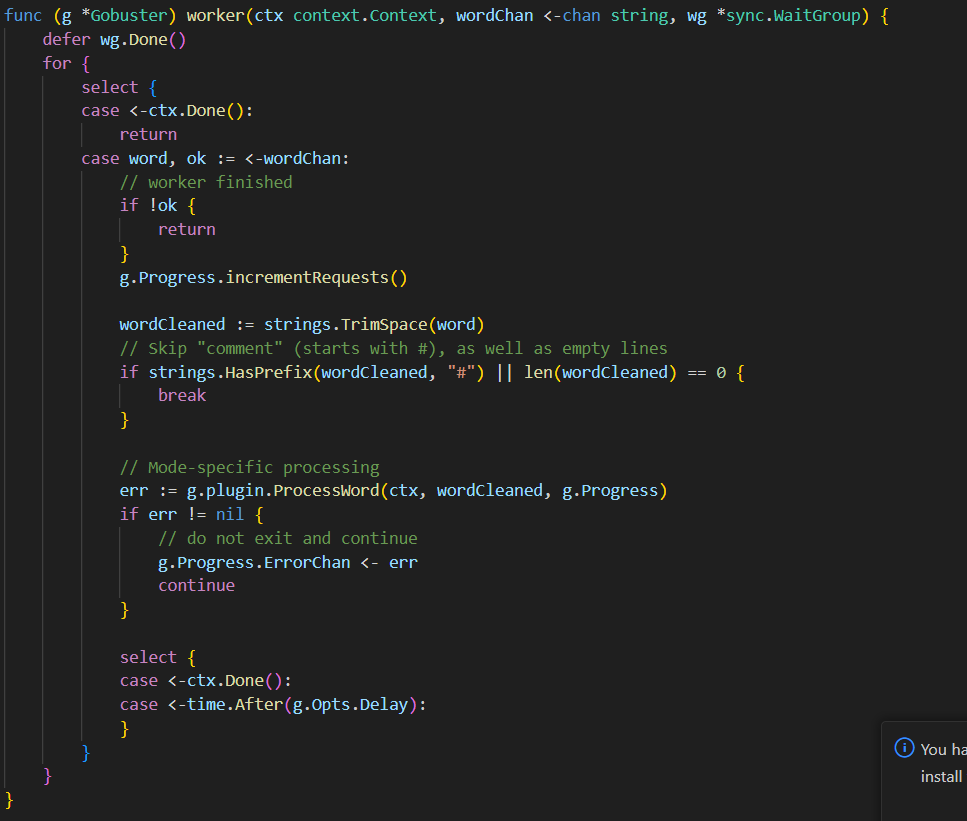
\includegraphics[width=0.4\textwidth]{Libgobuster_Worker.png}
    \caption{Worker function of a Gobuster Object}
    \label{fig: Libgobuster Worker}
\end{figure} \\
Besides, in the \textbf{http.go} file in this folder, an http connection is set up to send and receive data from the target url.\\
\begin{figure}[H]
    \centering
    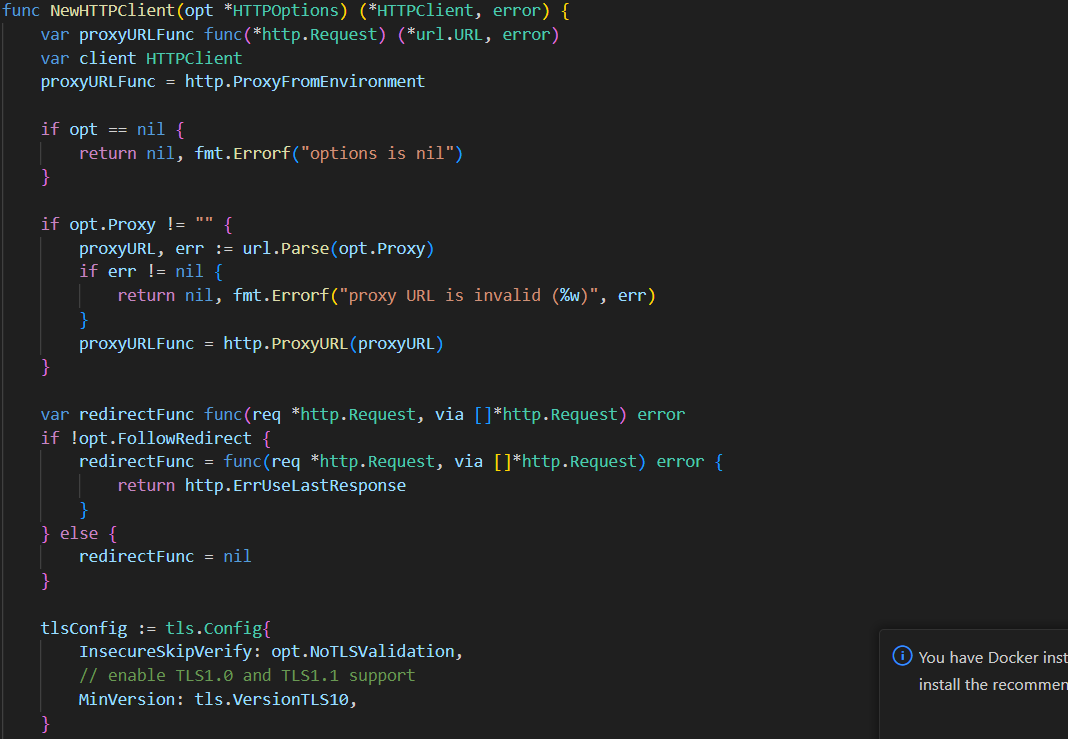
\includegraphics[width=0.4\textwidth]{HTTP_Connection.png}
    \caption{Setting up an http connection}
    \label{fig: HTTP Connection}
\end{figure}
\subsection{gobusterdir}
This mode is used to find hidden directories in a website. If we go to the file \textbf{gobusterdir.go} and view the \textbf{processWord} function, then we can see that it does the following:
\begin{itemize}
    \item It constructs the full URL by appending the given word from the word list to the base URL, like \textbf{example.com/word} format. It ensures that the base URL ends with a slash and removes any leading slashes from the word.
    \item It allows for multiple attempts in case of timeout errors based on the values of the flags.
    \begin{figure}[H]
        \centering
        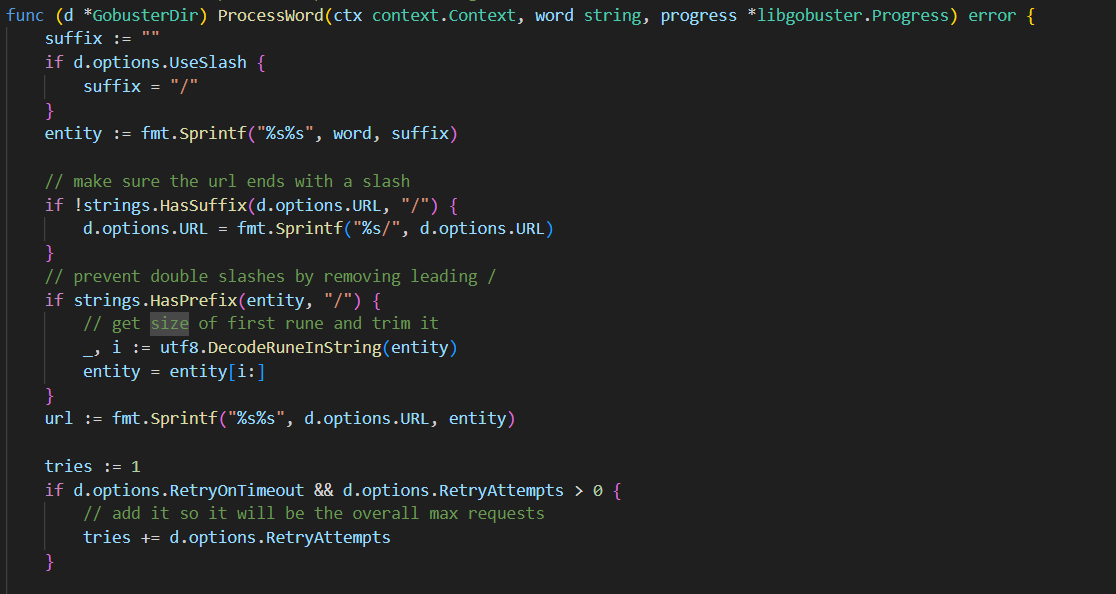
\includegraphics[width=0.4\textwidth]{Gobusterdir_Constructing_Url.png}
        \caption{Constructing URL in Directory mode}
        \label{fig: Directory Mode Constructing URL}
    \end{figure}
    \item Then the function sends an http request using \textbf{d.http.Request}.
    \item As a result, we get status code, size of response from the return value, and the result is sent to the result channel.
    \begin{figure}[H]
        \centering
        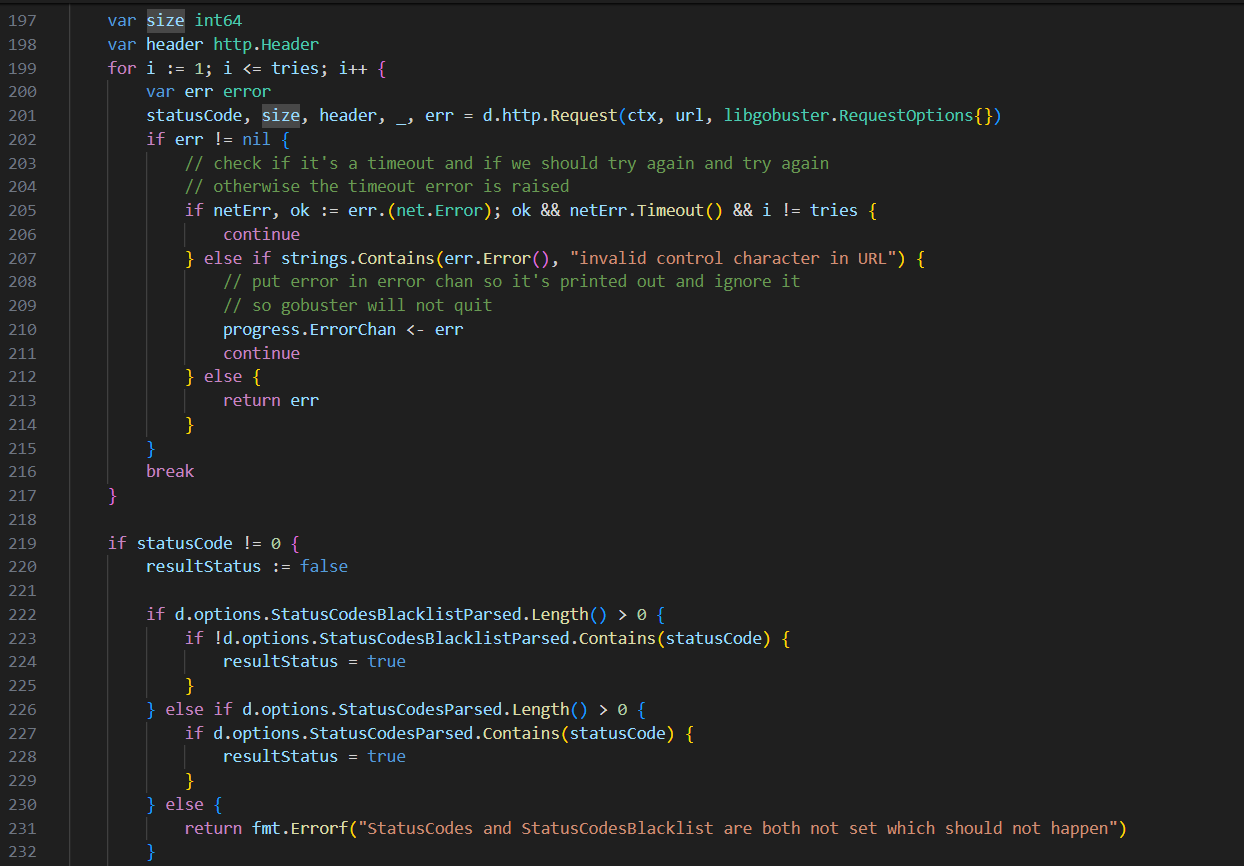
\includegraphics[width=0.4\textwidth]{Gobusterdir_Http_Request.png}
        \caption{Sending an http request in directory mode}
        \label{fig: Directory Mode HTTP Request}
    \end{figure}
\end{itemize}
\subsection{gobusterdns}
The DNS mode is used to find subdomains of a website. In DNS mode,
the tool appends words in front of the domain name and sends DNS queries to verify which subdomains exist. If we go to the file \textbf{gobusterdns.go} and view the \textbf{processWord} function, then we can see that it does the following:
\begin{figure}[H]
    \centering
    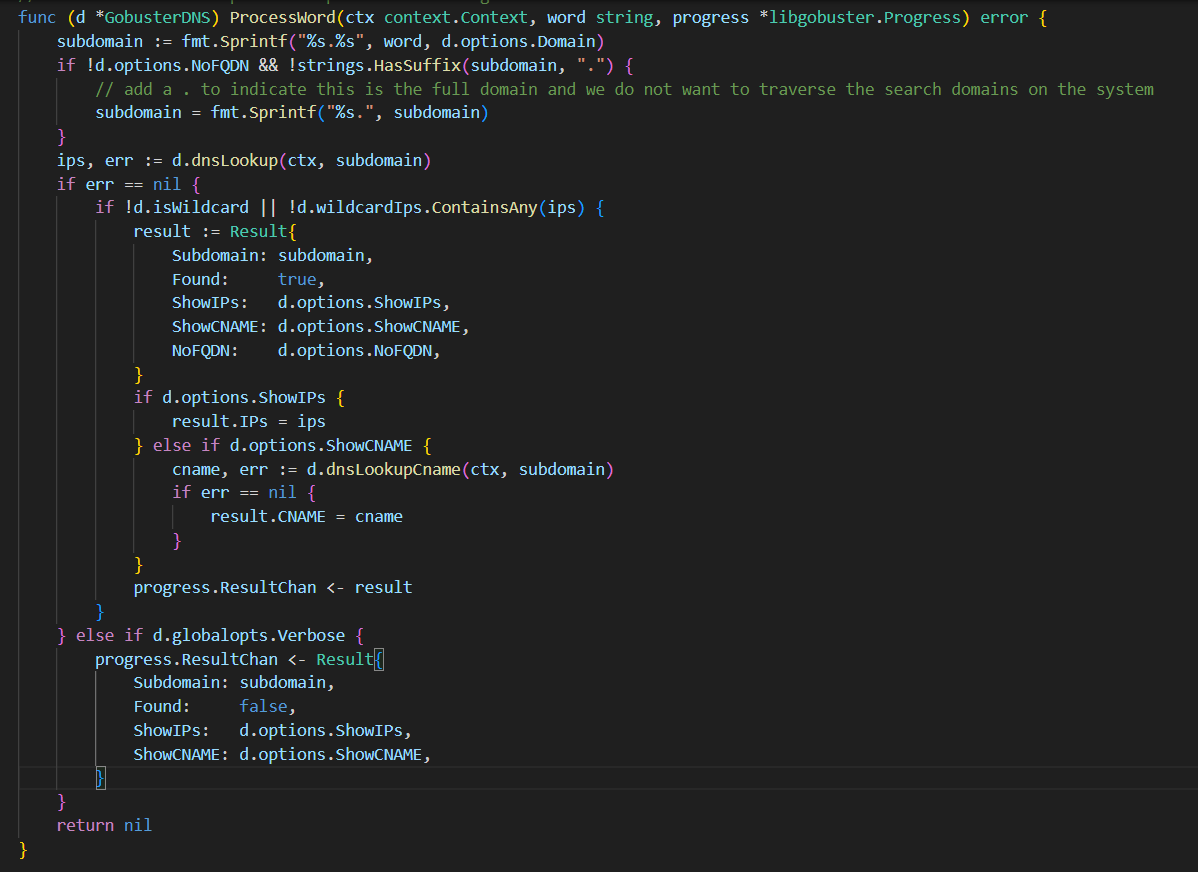
\includegraphics[width=0.4\textwidth]{Gobusterdns_ProcessWord.png}
    \caption{processWord function in DNS mode}
    \label{fig: Gobusterdns processWord}
\end{figure}
\begin{itemize}
    \item It constructs the subdomain by appending the current word to the specified Domain, like \textbf{word.example.com} format.
    \item It performs a DNS lookup for the constructed subdomain using the \textbf{dnsLookup} method. If there is no error, it checks for wildcards and ensures the subdomain is not part of the wildcard IPs.
    \item If \textbf{ShowIPs} option is enabled, it includes the resolved IPs in the result. Then it sends the results to the result channel.
    \item For each word in the wordlist, it either reports the successful resolution of the subdomain or, if in \textbf{Verbose} mode, reports when a subdomain is not found.
\end{itemize}
\subsection{gobustervhost}
For looking for sites that are hosted virtually by the same website, we send http requests to the same website with different hostname in header. If we go to the file \textbf{gobustervhost.go} and view the \textbf{processWord} function, then we can see that it does the following:
\begin{itemize}
    \item First it constructs the subdomain name from the given word file.
    \begin{figure}[H]
        \centering
        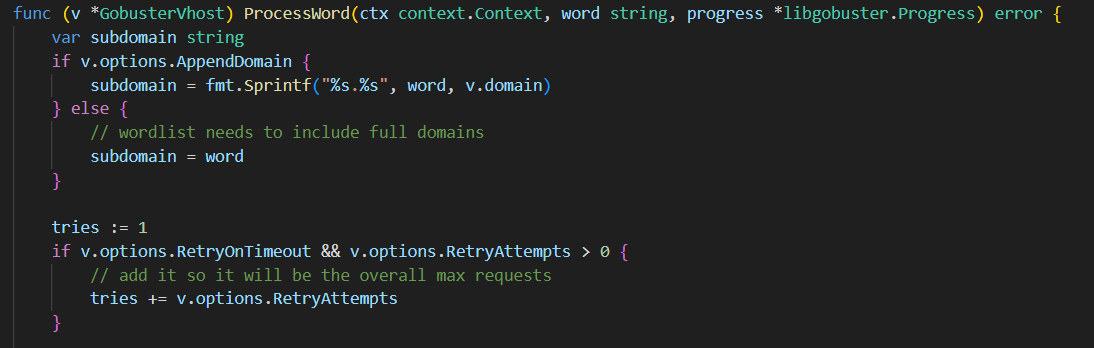
\includegraphics[width=0.4\textwidth]{Gobustervhost_Construct_Subdomain.png}
        \caption{Constructing Subdomain in vhost mode}
        \label{fig: Gobustervhost Constructing Subdomain}
    \end{figure}
    \item Then it sends an http request to the subdomain and gets response body, response size and status code as a response.
    \begin{figure}[H]
        \centering
        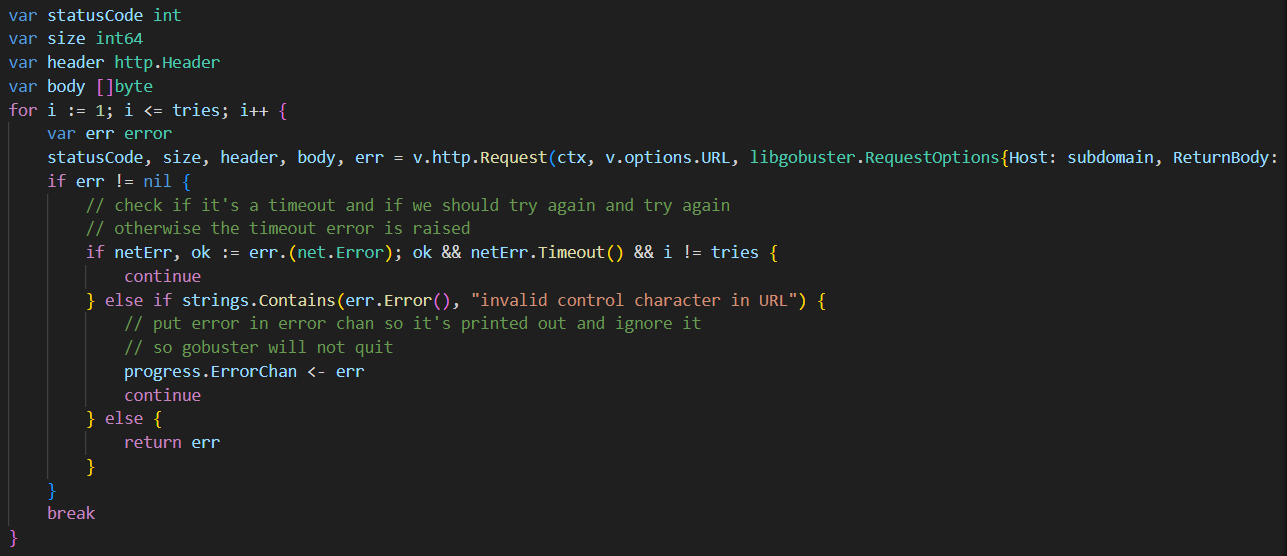
\includegraphics[width=0.4\textwidth]{Gobustervhost_Get_Response.png}
        \caption{Get Response in vhost mode}
        \label{fig: Gobustervhost Get Response}
    \end{figure}
    \item Now we need to see if the response body is the same as default response body or error response body. So, we send an http request to the domain name to get \textbf{normal body}. We also send abnormal request using a \textbf{uuid generator} and save the response body as \textbf{abnormal body}.
    \item Finally, we compare our response with normal and abnormal body. If there’s no match with either, we can be sure that the response body is from a different website. Thus, we get a new website hosted by the base domain.
    \begin{figure}[H]
        \centering
        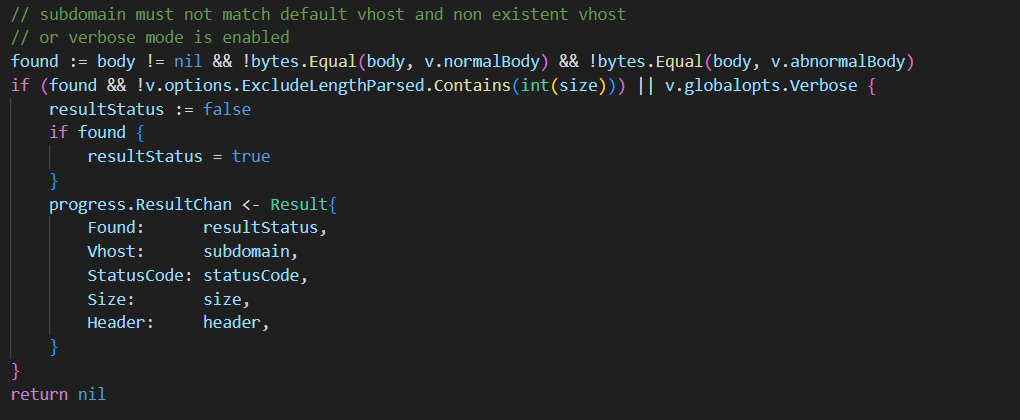
\includegraphics[width=0.4\textwidth]{Gobustervhost_Compare_Response.png}
        \caption{Compare Responses in vhost mode}
        \label{fig: Gobustervhost Compare Response}
    \end{figure}
\end{itemize}
\subsection{gobusterfuzz}
Fuzzing is the process of finding different parameters on a website.
In FUZZ mode, we can insert content from wordlists into different places of a website and check the responses to understand which parameters are valid for that website. If we go to the file \textbf{gobusterfuzz.go} and view the \textbf{processWord} function, then we can see that it does the following:
\begin{itemize}
    \item First, the function replaces the \textbf{FuzzKeyword} (a placeholder for the fuzzed payload) in the target URL with the current word from the wordlist.
    \begin{figure}[H]
        \centering
        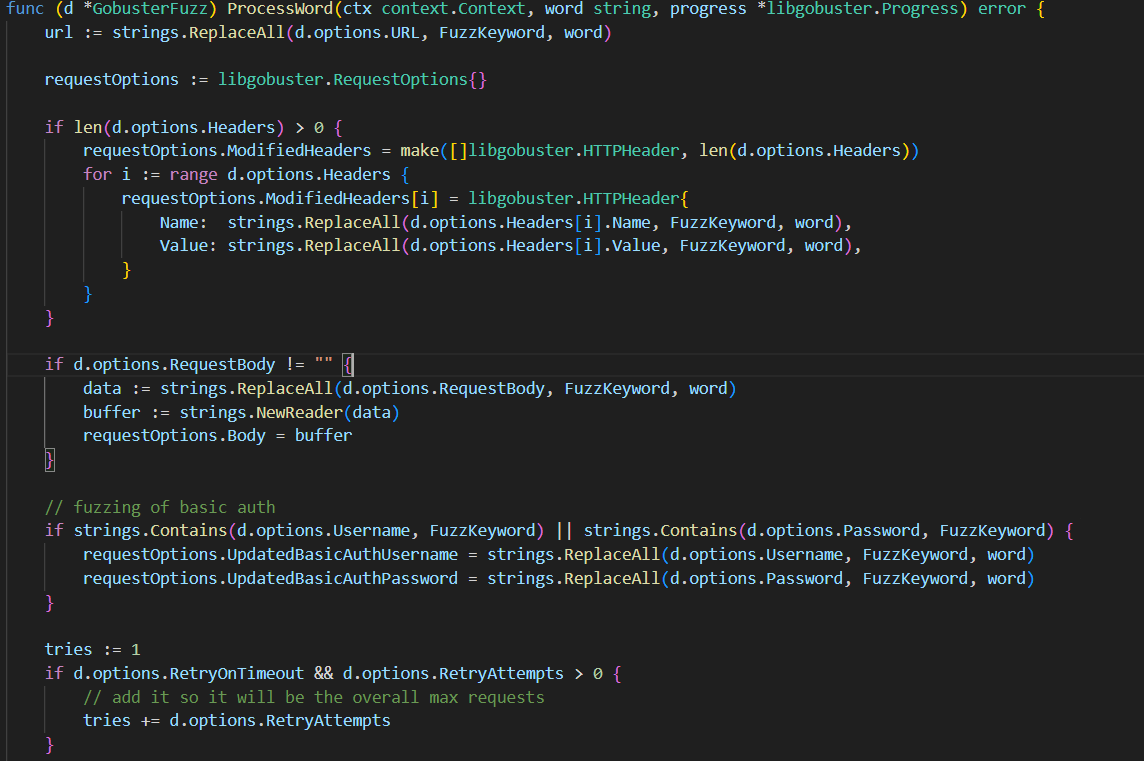
\includegraphics[width=0.4\textwidth]{Gobusterfuzz_Construct_Url.png}
        \caption{Constructing URL in fuzz mode}
        \label{fig: Gobusterfuzz Construct URL}
    \end{figure}
    \item Then it sends an http request to the target URL.
    \begin{figure}[H]
        \centering
        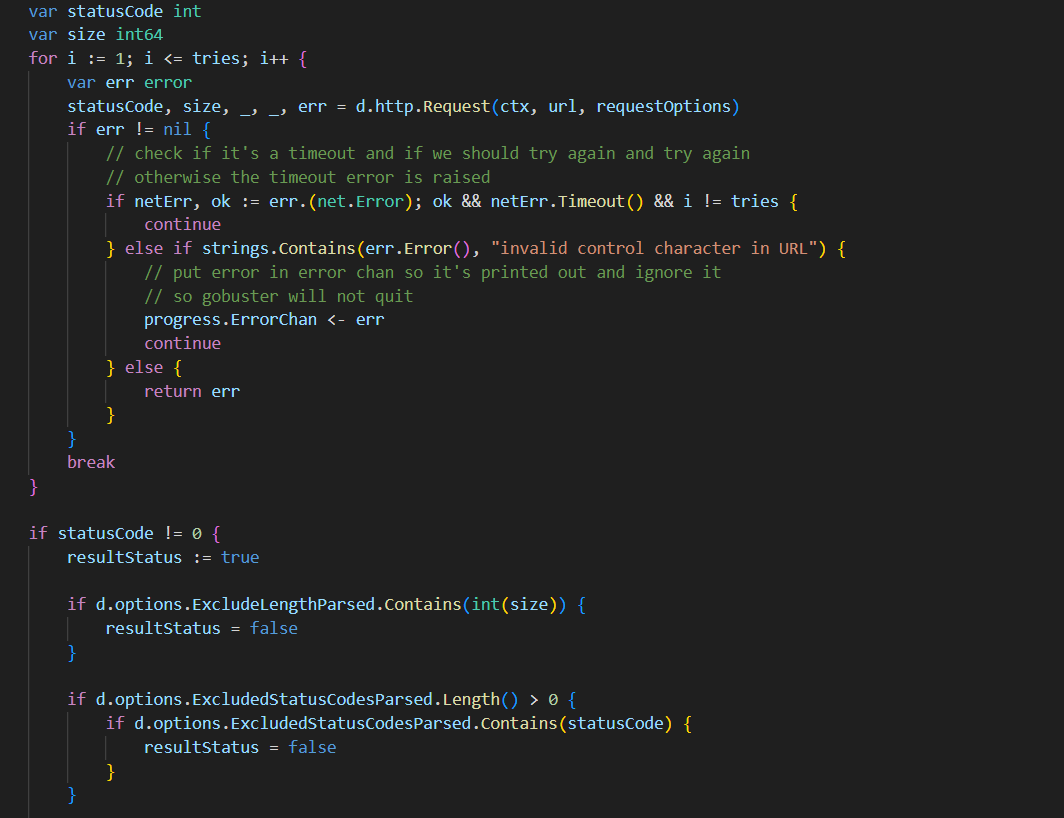
\includegraphics[width=0.4\textwidth]{Gobusterfuzz_Send_Request.png}
        \caption{Sending request in fuzz mode}
        \label{fig: Gobusterfuzz Send Request}
    \end{figure}
    \item We get the status code, response size and body. Upon examining these, we can determine which parameters are valid for the website.
\end{itemize}
\subsection{gobustergcs}
This mode is used to find publicly available gcs buckets. If we go to the file \textbf{gobustergcs.go} and view the \textbf{processWord} function, then we can see that it does the following:
\begin{itemize}
    \item First, the function constructs the target URL with the current word from the wordlist, like this \textbf{https://storage.googleapis.com/storage/v1/b/bucket/o} format.
    \item Then it sends an http request to the target URL.
    \begin{figure}[H]
        \centering
        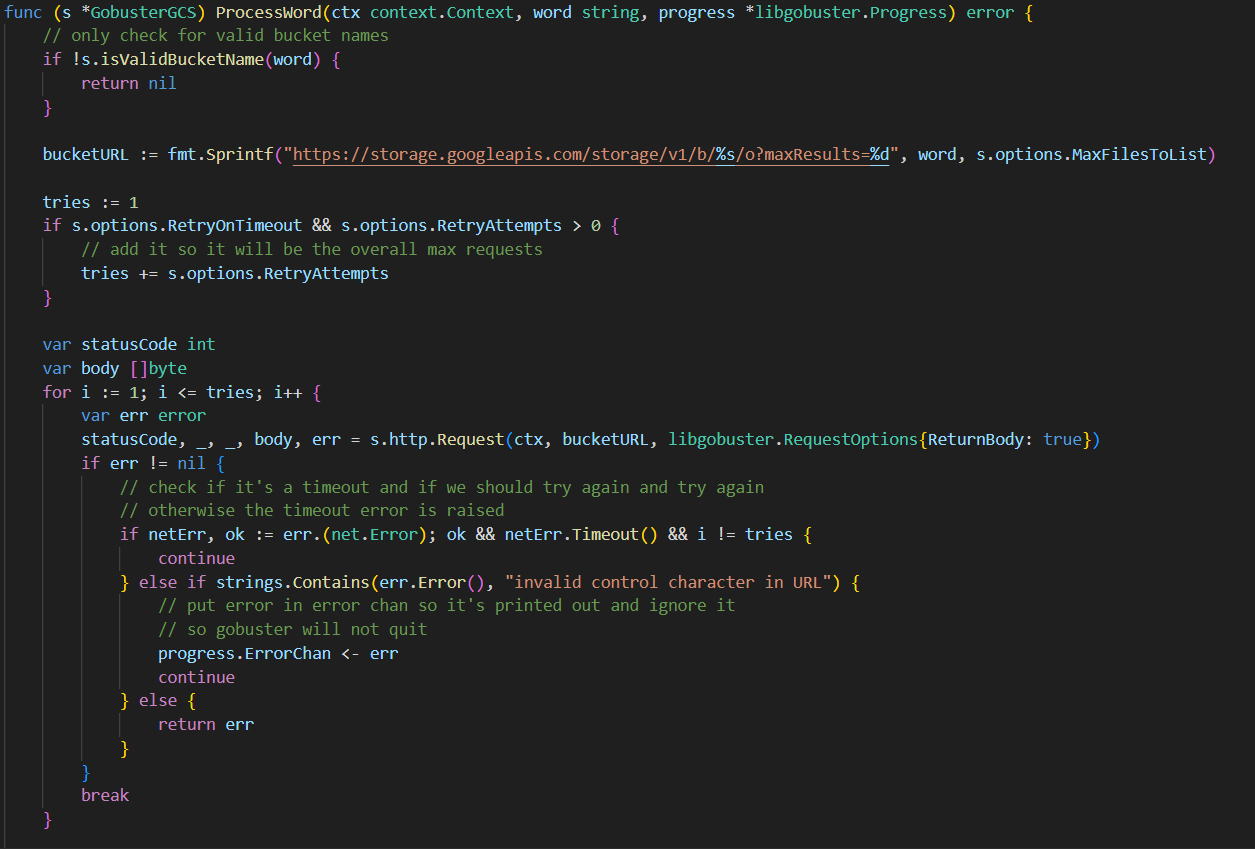
\includegraphics[width=0.4\textwidth]{Gobustergcs_processWord.png}
        \caption{Constructing URL and getting response in gcs mode}
        \label{fig: Gobustergcs processWord}
    \end{figure}
    \item We get the status code, response size and body. From there after clicking on the media links, we can find the publicly available gcs buckets.
\end{itemize}
\subsection{gobusters3}
This mode works almost identically to gcs. The difference is in the url that is required to access public S3 buckets of amazon. If we go to the file \textbf{gobusters3.go} and view the \textbf{processWord} function, then we can see that it does the following:
\begin{itemize}
    \item First, the function constructs the target URL with the current word from the wordlist, like this \textbf{https://bucket.s3.amazonaws.com/} format.
    \item Then it sends an http request to the target URL.
    \begin{figure}[H]
        \centering
        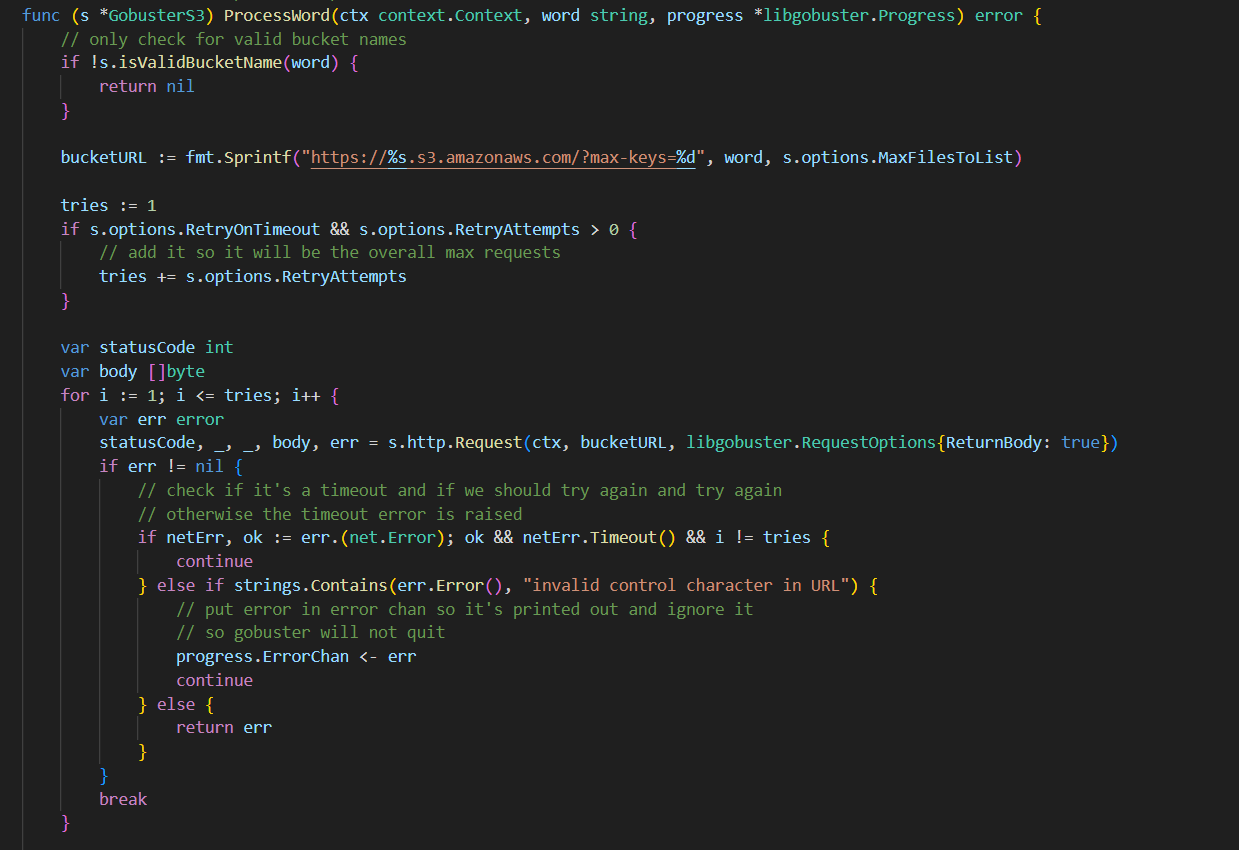
\includegraphics[width=0.4\textwidth]{Gobusters3_processWord.png}
        \caption{Constructing URL and getting response in s3 mode}
        \label{fig: Gobusters3 processWord}
    \end{figure}
    \item We get the status code, response size and body. From there we can visit the links and see which files are accessible.
\end{itemize}
\subsection{gobustertftp}
Tftp servers are a type of ftp servers, but with less protection. Tftp servers don’t require any password to access them. We can use brute forcing of gobuster to find some filenames in a particular tftp server. If we go to the file \textbf{gobustertftp.go} and view the \textbf{processWord} function, then we can see that it does the following:
\begin{itemize}
    \item First, the client is connected to the given server address.
    \item Then we enumerate our word file for words and send an http request to the server to find the target file with the same name there.
    \begin{figure}[H]
        \centering
        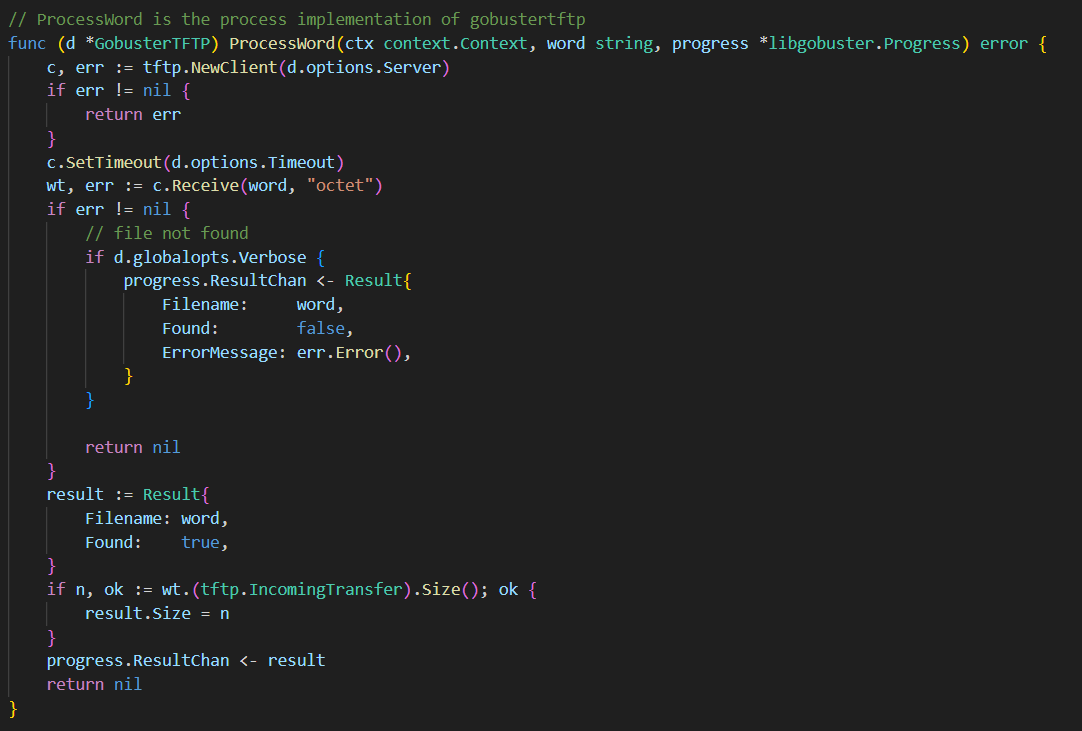
\includegraphics[width=0.4\textwidth]{Gobustertftp_processWord.png}
        \caption{Connecting to server and getting response in tftp mode}
        \label{fig: Gobustertftp processWord}
    \end{figure}
    \item As tftp does not have any protection, we can get the files by the same name returned. Thus, we can find the files in our tftp server.
\end{itemize}
\section{Documentation}
Running the features in gobuster is very straightforward. We just need to run the commands for the specific mode in gobuster. We can see the basic modes of operation using the \textbf{gobuster --help} command.\\ 
\begin{lstlisting}[language=bash]
$ gobuster --help                             
Usage:
  gobuster [command]

Available Commands:
  completion  Generate the autocompletion script for the specified shell
  dir         Uses directory/file enumeration mode
  dns         Uses DNS subdomain enumeration mode
  fuzz        Uses fuzzing mode. Replaces the keyword FUZZ in the URL, Headers and the request body
  gcs         Uses gcs bucket enumeration mode
  help        Help about any command
  s3          Uses aws bucket enumeration mode
  tftp        Uses TFTP enumeration mode
  version     shows the current version
  vhost       Uses VHOST enumeration mode (you most probably want to use the IP address as the URL parameter)

Flags:
      --debug                 Enable debug output
      --delay duration        Time each thread waits between requests (e.g. 1500ms)
  -h, --help                  help for gobuster
      --no-color              Disable color output
      --no-error              Don't display errors
  -z, --no-progress           Don't display progress
  -o, --output string         Output file to write results to (defaults to stdout)
  -p, --pattern string        File containing replacement patterns
  -q, --quiet                 Don't print the banner and other noise
  -t, --threads int           Number of concurrent threads (default 10)
  -v, --verbose               Verbose output (errors)
  -w, --wordlist string       Path to the wordlist. Set to - to use STDIN.
      --wordlist-offset int   Resume from a given position in the wordlist (defaults to 0)
\end{lstlisting}

\subsection{DIR}
The basic structure of dir mode is given below:
\begin{lstlisting}[language=bash]
gobuster dir -u https://example.com -w parameters.txt
\end{lstlisting}
\begin{itemize}
    \item dir: DIR mode of operation
    \item -u: The URL string
    \item -w: Path to the wordlist file 
\end{itemize}
We can find more about the flags using the command \textbf{gobuster dir --help}
\begin{lstlisting}[language=bash]
$ gobuster dir --help
Uses directory/file enumeration mode

Usage:
  gobuster dir [flags]

Flags:
  -f, --add-slash                         Append / to each request
      --client-cert-p12 string            a p12 file to use for options TLS client certificates
      --client-cert-p12-password string   the password to the p12 file
      --client-cert-pem string            public key in PEM format for optional TLS client certificates
      --client-cert-pem-key string        private key in PEM format for optional TLS client certificates (this key needs to have no password)
  -c, --cookies string                    Cookies to use for the requests
  -d, --discover-backup                   Also search for backup files by appending multiple backup extensions
      --exclude-length string             exclude the following content lengths (completely ignores the status). You can separate multiple lengths by comma and it also supports ranges like 203-206
  -e, --expanded                          Expanded mode, print full URLs
  -x, --extensions string                 File extension(s) to search for
  -X, --extensions-file string            Read file extension(s) to search from the file
  -r, --follow-redirect                   Follow redirects
  -H, --headers stringArray               Specify HTTP headers, -H 'Header1: val1' -H 'Header2: val2'
  -h, --help                              help for dir
      --hide-length                       Hide the length of the body in the output
  -m, --method string                     Use the following HTTP method (default "GET")
      --no-canonicalize-headers           Do not canonicalize HTTP header names. If set header names are sent as is.
  -n, --no-status                         Don't print status codes
  -k, --no-tls-validation                 Skip TLS certificate verification
  -P, --password string                   Password for Basic Auth
      --proxy string                      Proxy to use for requests [http(s)://host:port] or [socks5://host:port]
      --random-agent                      Use a random User-Agent string
      --retry                             Should retry on request timeout
      --retry-attempts int                Times to retry on request timeout (default 3)
  -s, --status-codes string               Positive status codes (will be overwritten with status-codes-blacklist if set). Can also handle ranges like 200,300-400,404.
  -b, --status-codes-blacklist string     Negative status codes (will override status-codes if set). Can also handle ranges like 200,300-400,404. (default "404")
      --timeout duration                  HTTP Timeout (default 10s)
  -u, --url string                        The target URL
  -a, --useragent string                  Set the User-Agent string (default "gobuster/3.6")
  -U, --username string                   Username for Basic Auth

Global Flags:
      --debug                 Enable debug output
      --delay duration        Time each thread waits between requests (e.g. 1500ms)
      --no-color              Disable color output
      --no-error              Don't display errors
  -z, --no-progress           Don't display progress
  -o, --output string         Output file to write results to (defaults to stdout)
  -p, --pattern string        File containing replacement patterns
  -q, --quiet                 Don't print the banner and other noise
  -t, --threads int           Number of concurrent threads (default 10)
  -v, --verbose               Verbose output (errors)
  -w, --wordlist string       Path to the wordlist. Set to - to use STDIN.
      --wordlist-offset int   Resume from a given position in the wordlist (defaults to 0)
\end{lstlisting}
\subsection{DNS}
The basic structure of dns mode is given below:
\begin{lstlisting}[language=bash]
gobuster dns -d example.com -w subdomains.txt
\end{lstlisting}
\begin{itemize}
    \item dns: DNS mode of operation
    \item -d: The base URL string
    \item -w: Path to the wordlist file 
\end{itemize}
We can find more about the flags using the command \textbf{gobuster dns --help}
\begin{lstlisting}[language=bash]
$ gobuster dns --help
Uses DNS subdomain enumeration mode

Usage:
  gobuster dns [flags]

Flags:
  -d, --domain string      The target domain
  -h, --help               help for dns
      --no-fqdn            Do not automatically add a trailing dot to the domain, so the resolver uses the DNS search domain
  -r, --resolver string    Use custom DNS server (format server.com or server.com:port)
  -c, --show-cname         Show CNAME records (cannot be used with '-i' option)
  -i, --show-ips           Show IP addresses
      --timeout duration   DNS resolver timeout (default 1s)
      --wildcard           Force continued operation when wildcard found

Global Flags:
      --debug                 Enable debug output
      --delay duration        Time each thread waits between requests (e.g. 1500ms)
      --no-color              Disable color output
      --no-error              Don't display errors
  -z, --no-progress           Don't display progress
  -o, --output string         Output file to write results to (defaults to stdout)
  -p, --pattern string        File containing replacement patterns
  -q, --quiet                 Don't print the banner and other noise
  -t, --threads int           Number of concurrent threads (default 10)
  -v, --verbose               Verbose output (errors)
  -w, --wordlist string       Path to the wordlist. Set to - to use STDIN.
      --wordlist-offset int   Resume from a given position in the wordlist (defaults to 0)
\end{lstlisting}
\subsection{VHOST}
The basic structure of vhost mode is given below:
\begin{lstlisting}[language=bash]
gobuster vhost -u https://example.com -w words.txt
\end{lstlisting}
\begin{itemize}
    \item vhost: VHOST mode of operation
    \item -u: The base URL string
    \item -w: Path to the wordlist file 
\end{itemize}
We can find more about the flags using the command \textbf{gobuster vhost --help}
\begin{lstlisting}[language=bash]
$ gobuster vhost --help
Uses VHOST enumeration mode (you most probably want to use the IP address as the URL parameter)

Usage:
  gobuster vhost [flags]

Flags:
      --append-domain                     Append main domain from URL to words from wordlist. Otherwise the fully qualified domains need to be specified in the wordlist.
      --client-cert-p12 string            a p12 file to use for options TLS client certificates
      --client-cert-p12-password string   the password to the p12 file
      --client-cert-pem string            public key in PEM format for optional TLS client certificates
      --client-cert-pem-key string        private key in PEM format for optional TLS client certificates (this key needs to have no password)
  -c, --cookies string                    Cookies to use for the requests
      --domain string                     the domain to append when using an IP address as URL. If left empty and you specify a domain based URL the hostname from the URL is extracted
      --exclude-length string             exclude the following content lengths (completely ignores the status). You can separate multiple lengths by comma and it also supports ranges like 203-206
  -r, --follow-redirect                   Follow redirects
  -H, --headers stringArray               Specify HTTP headers, -H 'Header1: val1' -H 'Header2: val2'
  -h, --help                              help for vhost
  -m, --method string                     Use the following HTTP method (default "GET")
      --no-canonicalize-headers           Do not canonicalize HTTP header names. If set header names are sent as is.
  -k, --no-tls-validation                 Skip TLS certificate verification
  -P, --password string                   Password for Basic Auth
      --proxy string                      Proxy to use for requests [http(s)://host:port] or [socks5://host:port]
      --random-agent                      Use a random User-Agent string
      --retry                             Should retry on request timeout
      --retry-attempts int                Times to retry on request timeout (default 3)
      --timeout duration                  HTTP Timeout (default 10s)
  -u, --url string                        The target URL
  -a, --useragent string                  Set the User-Agent string (default "gobuster/3.6")
  -U, --username string                   Username for Basic Auth

Global Flags:
      --debug                 Enable debug output
      --delay duration        Time each thread waits between requests (e.g. 1500ms)
      --no-color              Disable color output
      --no-error              Don't display errors
  -z, --no-progress           Don't display progress
  -o, --output string         Output file to write results to (defaults to stdout)
  -p, --pattern string        File containing replacement patterns
  -q, --quiet                 Don't print the banner and other noise
  -t, --threads int           Number of concurrent threads (default 10)
  -v, --verbose               Verbose output (errors)
  -w, --wordlist string       Path to the wordlist. Set to - to use STDIN.
      --wordlist-offset int   Resume from a given position in the wordlist (defaults to 0)
\end{lstlisting}
\subsection{FUZZ}
The basic structure of fuzz mode is given below:
\begin{lstlisting}[language=bash]
gobuster fuzz -u https://example.com?FUZZ=test -w parameters.txt
\end{lstlisting}
\begin{itemize}
    \item fuzz: FUZZ mode of operation
    \item -u: The URL string
    \item -w: Path to the wordlist file 
\end{itemize}
We can find more about the flags using the command \textbf{gobuster fuzz --help}
\begin{lstlisting}[language=bash]
$ gobuster fuzz --help                                                                                                                                                 
Uses fuzzing mode. Replaces the keyword FUZZ in the URL, Headers and the request body

Usage:
  gobuster fuzz [flags]

Flags:
  -B, --body string                       Request body
      --client-cert-p12 string            a p12 file to use for options TLS client certificates
      --client-cert-p12-password string   the password to the p12 file
      --client-cert-pem string            public key in PEM format for optional TLS client certificates
      --client-cert-pem-key string        private key in PEM format for optional TLS client certificates (this key needs to have no password)
  -c, --cookies string                    Cookies to use for the requests
      --exclude-length string             exclude the following content lengths (completely ignores the status). You can separate multiple lengths by comma and it also supports ranges like 203-206
  -b, --excludestatuscodes string         Excluded status codes. Can also handle ranges like 200,300-400,404.
  -r, --follow-redirect                   Follow redirects
  -H, --headers stringArray               Specify HTTP headers, -H 'Header1: val1' -H 'Header2: val2'
  -h, --help                              help for fuzz
  -m, --method string                     Use the following HTTP method (default "GET")
      --no-canonicalize-headers           Do not canonicalize HTTP header names. If set header names are sent as is.
  -k, --no-tls-validation                 Skip TLS certificate verification
  -P, --password string                   Password for Basic Auth
      --proxy string                      Proxy to use for requests [http(s)://host:port] or [socks5://host:port]
      --random-agent                      Use a random User-Agent string
      --retry                             Should retry on request timeout
      --retry-attempts int                Times to retry on request timeout (default 3)
      --timeout duration                  HTTP Timeout (default 10s)
  -u, --url string                        The target URL
  -a, --useragent string                  Set the User-Agent string (default "gobuster/3.6")
  -U, --username string                   Username for Basic Auth

Global Flags:
      --debug                 Enable debug output
      --delay duration        Time each thread waits between requests (e.g. 1500ms)
      --no-color              Disable color output
      --no-error              Don't display errors
  -z, --no-progress           Don't display progress
  -o, --output string         Output file to write results to (defaults to stdout)
  -p, --pattern string        File containing replacement patterns
  -q, --quiet                 Don't print the banner and other noise
  -t, --threads int           Number of concurrent threads (default 10)
  -v, --verbose               Verbose output (errors)
  -w, --wordlist string       Path to the wordlist. Set to - to use STDIN.
      --wordlist-offset int   Resume from a given position in the wordlist (defaults to 0)
\end{lstlisting}

\subsection{GCS}
The basic structure of gcs mode is given below:
\begin{lstlisting}[language=bash]
gobuster gcs -w bucket-names.txt
\end{lstlisting}
\begin{itemize}
    \item gcs: gcs mode of operation
    \item -w: Path to the wordlist file 
\end{itemize}
We can find more about the flags using the command \textbf{gobuster gcs --help}
\begin{lstlisting}[language=bash]
$ gobuster gcs --help                                                                                                                                                  
Uses gcs bucket enumeration mode

Usage:
  gobuster gcs [flags]

Flags:
      --client-cert-p12 string            a p12 file to use for options TLS client certificates
      --client-cert-p12-password string   the password to the p12 file
      --client-cert-pem string            public key in PEM format for optional TLS client certificates
      --client-cert-pem-key string        private key in PEM format for optional TLS client certificates (this key needs to have no password)
  -h, --help                              help for gcs
  -m, --maxfiles int                      max files to list when listing buckets (only shown in verbose mode) (default 5)
  -k, --no-tls-validation                 Skip TLS certificate verification
      --proxy string                      Proxy to use for requests [http(s)://host:port] or [socks5://host:port]
      --random-agent                      Use a random User-Agent string
      --retry                             Should retry on request timeout
      --retry-attempts int                Times to retry on request timeout (default 3)
      --timeout duration                  HTTP Timeout (default 10s)
  -a, --useragent string                  Set the User-Agent string (default "gobuster/3.6")

Global Flags:
      --debug                 Enable debug output
      --delay duration        Time each thread waits between requests (e.g. 1500ms)
      --no-color              Disable color output
      --no-error              Don't display errors
  -z, --no-progress           Don't display progress
  -o, --output string         Output file to write results to (defaults to stdout)
  -p, --pattern string        File containing replacement patterns
  -q, --quiet                 Don't print the banner and other noise
  -t, --threads int           Number of concurrent threads (default 10)
  -v, --verbose               Verbose output (errors)
  -w, --wordlist string       Path to the wordlist. Set to - to use STDIN.
      --wordlist-offset int   Resume from a given position in the wordlist (defaults to 0)
\end{lstlisting}

\subsection{S3}
The basic structure of s3 mode is given below:
\begin{lstlisting}[language=bash]
gobuster s3 -w bucket-names.txt
\end{lstlisting}
\begin{itemize}
    \item s3: s3 mode of operation
    \item -w: Path to the wordlist file 
\end{itemize}
We can find more about the flags using the command \textbf{gobuster s3 --help}
\begin{lstlisting}[language=bash]
$ gobuster s3 --help 
Uses aws bucket enumeration mode

Usage:
  gobuster s3 [flags]

Flags:
      --client-cert-p12 string            a p12 file to use for options TLS client certificates
      --client-cert-p12-password string   the password to the p12 file
      --client-cert-pem string            public key in PEM format for optional TLS client certificates
      --client-cert-pem-key string        private key in PEM format for optional TLS client certificates (this key needs to have no password)
  -h, --help                              help for s3
  -m, --maxfiles int                      max files to list when listing buckets (only shown in verbose mode) (default 5)
  -k, --no-tls-validation                 Skip TLS certificate verification
      --proxy string                      Proxy to use for requests [http(s)://host:port] or [socks5://host:port]
      --random-agent                      Use a random User-Agent string
      --retry                             Should retry on request timeout
      --retry-attempts int                Times to retry on request timeout (default 3)
      --timeout duration                  HTTP Timeout (default 10s)
  -a, --useragent string                  Set the User-Agent string (default "gobuster/3.6")

Global Flags:
      --debug                 Enable debug output
      --delay duration        Time each thread waits between requests (e.g. 1500ms)
      --no-color              Disable color output
      --no-error              Don't display errors
  -z, --no-progress           Don't display progress
  -o, --output string         Output file to write results to (defaults to stdout)
  -p, --pattern string        File containing replacement patterns
  -q, --quiet                 Don't print the banner and other noise
  -t, --threads int           Number of concurrent threads (default 10)
  -v, --verbose               Verbose output (errors)
  -w, --wordlist string       Path to the wordlist. Set to - to use STDIN.
      --wordlist-offset int   Resume from a given position in the wordlist (defaults to 0)
\end{lstlisting}
\subsection{TFTP}
The basic structure of tftp mode is given below:
\begin{lstlisting}[language=bash]
gobuster tftp -s tftp.example.com -w common-filenames.txt
\end{lstlisting}
\begin{itemize}
    \item tftp: tftp mode of operation
    \item -s: The target tftp server 
    \item -w: Path to the wordlist file
\end{itemize}
We can find more about the flags using the command \textbf{gobuster tftp --help}
\begin{lstlisting}[language=bash]
$ gobuster tftp --help
Uses TFTP enumeration mode

Usage:
  gobuster tftp [flags]

Flags:
  -h, --help               help for tftp
  -s, --server string      The target TFTP server
      --timeout duration   TFTP timeout (default 1s)

Global Flags:
      --debug                 Enable debug output
      --delay duration        Time each thread waits between requests (e.g. 1500ms)
      --no-color              Disable color output
      --no-error              Don't display errors
  -z, --no-progress           Don't display progress
  -o, --output string         Output file to write results to (defaults to stdout)
  -p, --pattern string        File containing replacement patterns
  -q, --quiet                 Don't print the banner and other noise
  -t, --threads int           Number of concurrent threads (default 10)
  -v, --verbose               Verbose output (errors)
  -w, --wordlist string       Path to the wordlist. Set to - to use STDIN.
      --wordlist-offset int   Resume from a given position in the wordlist (defaults to 0)
\end{lstlisting}

\section{Demonstration}
We will see some demonstration of the 7 different modes of gobuster.
\subsection{DIR}
In the directory mode, we scan for hidden directories and vulnerable files in the websites. A demonstration of directory busting:
\textbf{\underline{First Example:}}
\begin{lstlisting}
$ gobuster dir -u https://cse.buet.ac.bd -w test_wordlist.txt -t 25 
\end{lstlisting}
Here we are searching for vulnerable files in cse.buet.ac.bd.
The output files are below:
\begin{figure}[H]
    \centering
    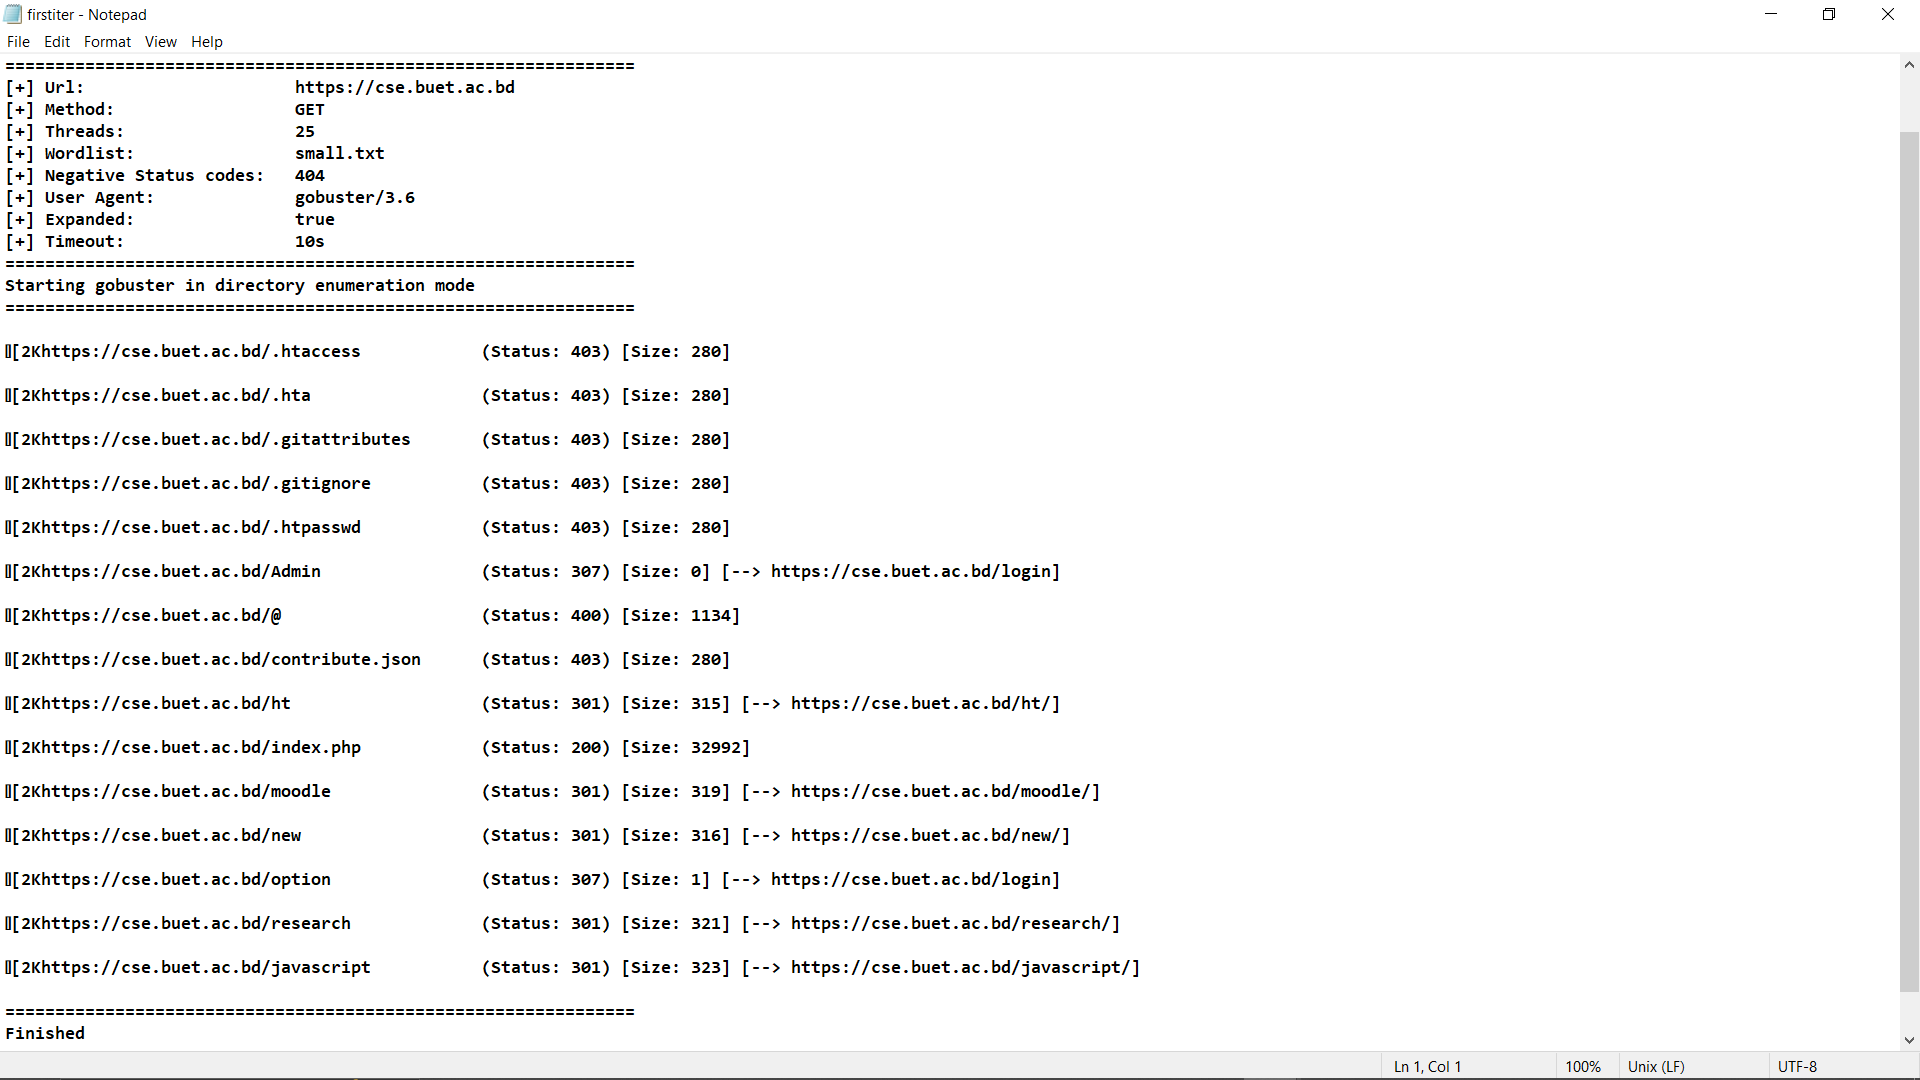
\includegraphics[width=0.7\textwidth]{dir_1.png}
    \caption{Output of the dir mode on cse.buet.ac.bd}
    \label{fig: dir Output}
\end{figure}
We get cse.buet.ac.bd/javascript. If we further scan cse.buet.ac.bd/javascript, we get the following output:
\begin{figure}[H]
    \centering
    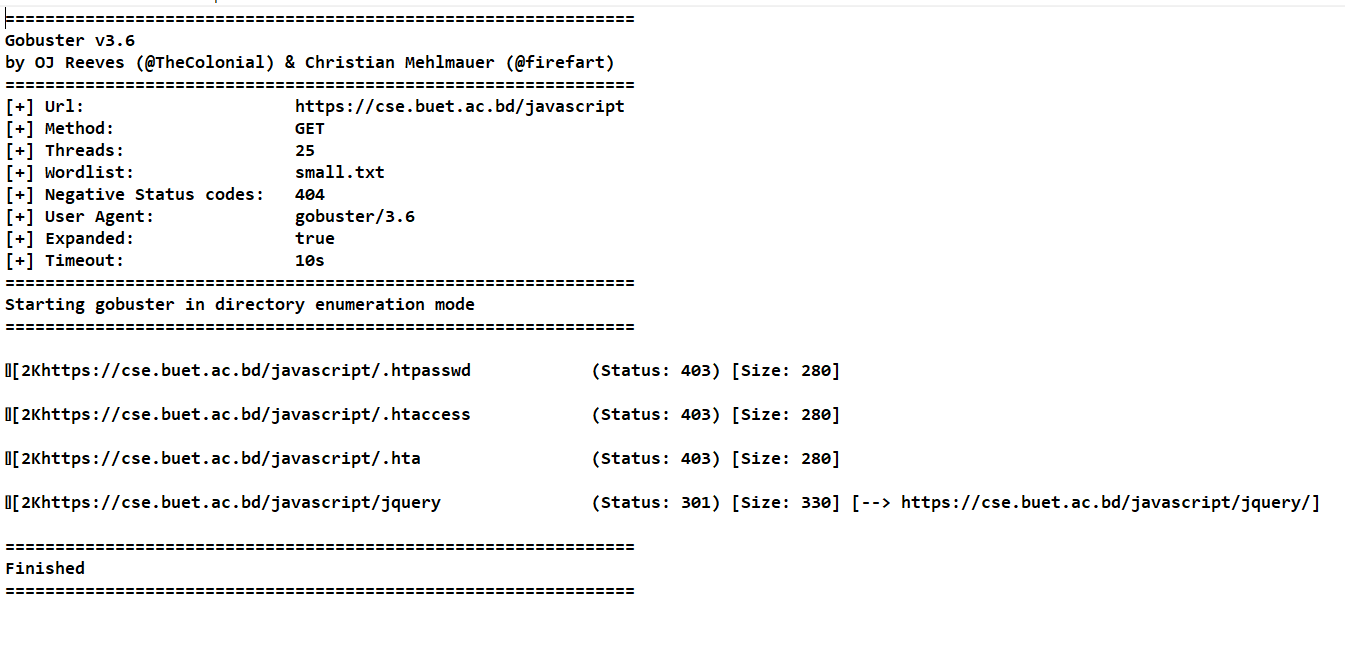
\includegraphics[width=0.7\textwidth]{dir_2.png}
    \caption{Output of the dir mode on cse.buet.ac.bd/javascript}
    \label{fig: dir2 Output}
\end{figure}
If we scan further on cse.buet.ac.bd/javascript/jquery, then we get the following output:
\begin{figure}[H]
    \centering
    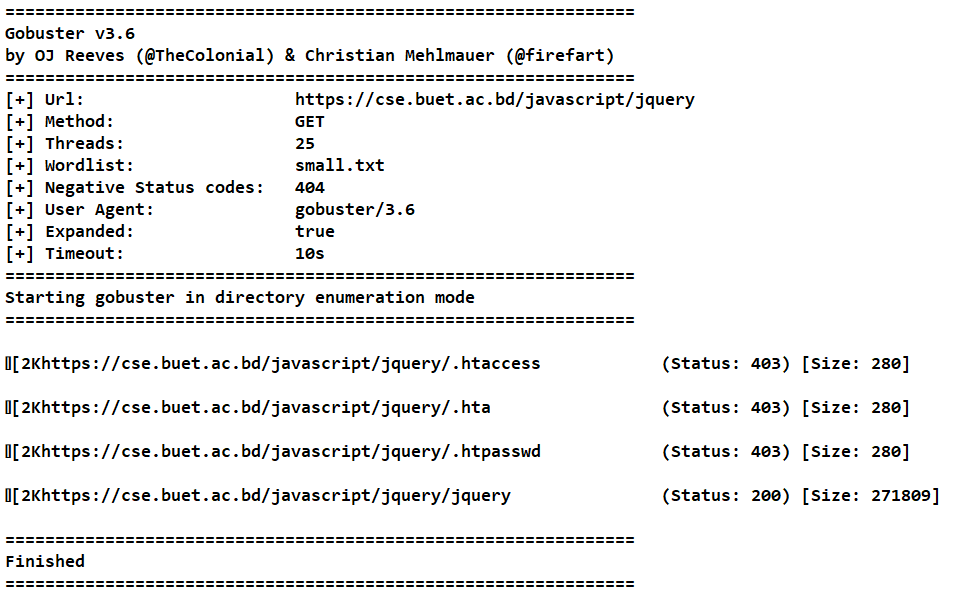
\includegraphics[width=0.7\textwidth]{dir_3.png}
    \caption{Output of the dir mode on cse.buet.ac.bd/javascript/jquery}
    \label{fig: dir3 Output}
\end{figure}
We got a hidden file cse.buet.ac.bd/javascript/jquery/jquery which can be accessed. If we access the url, we get:
\begin{figure}[H]
    \centering
    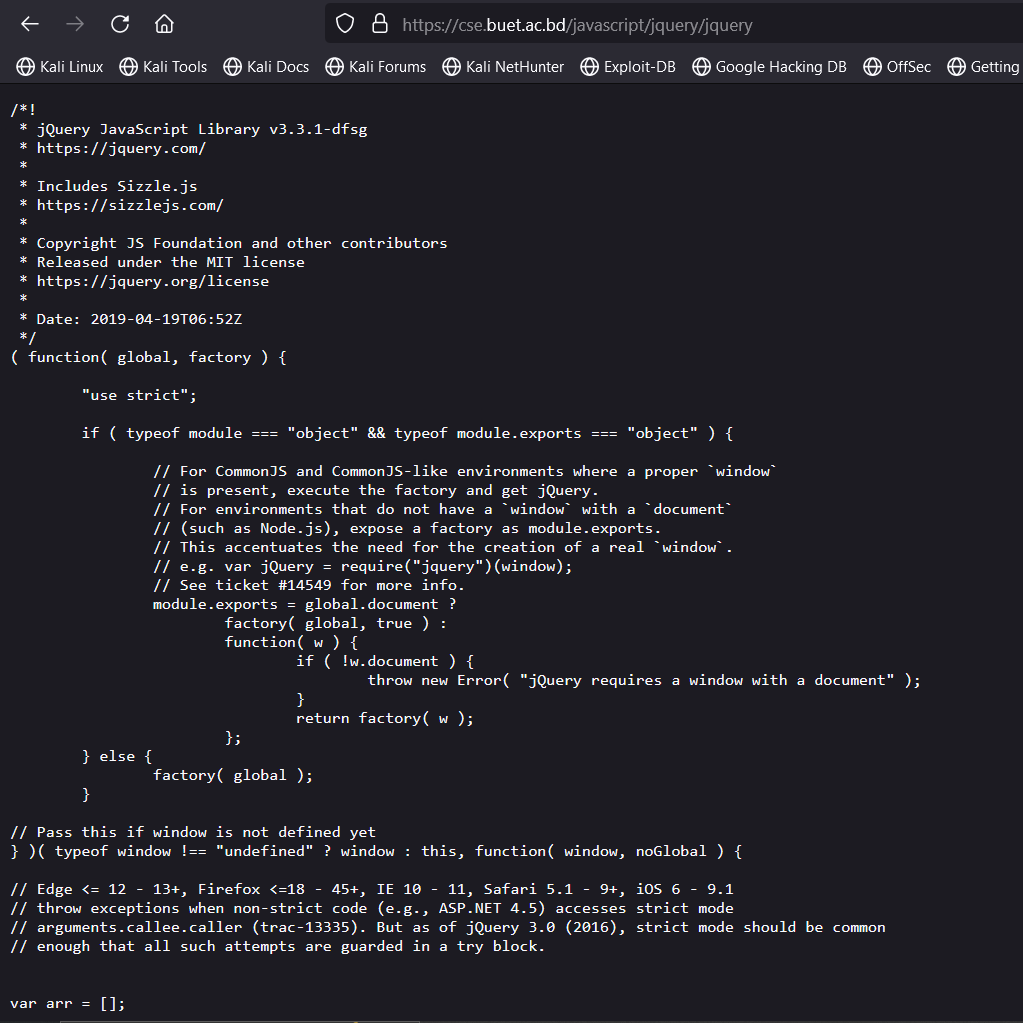
\includegraphics[width=0.5\textwidth]{dir_4.png}
    \caption{Accessing cse.buet.ac.bd/javascript/jquery/jquery}
    \label{fig: dir4 Output}
\end{figure}
\textbf{\underline{Second Example:}}
We will now solve a ctf problem using gobuster. We can find the problem statement here: \href{https://gobustme.ctflearn.com/}{Problem}\\ \\
We can get a look at the problem too.
\begin{figure}[H]
    \centering
    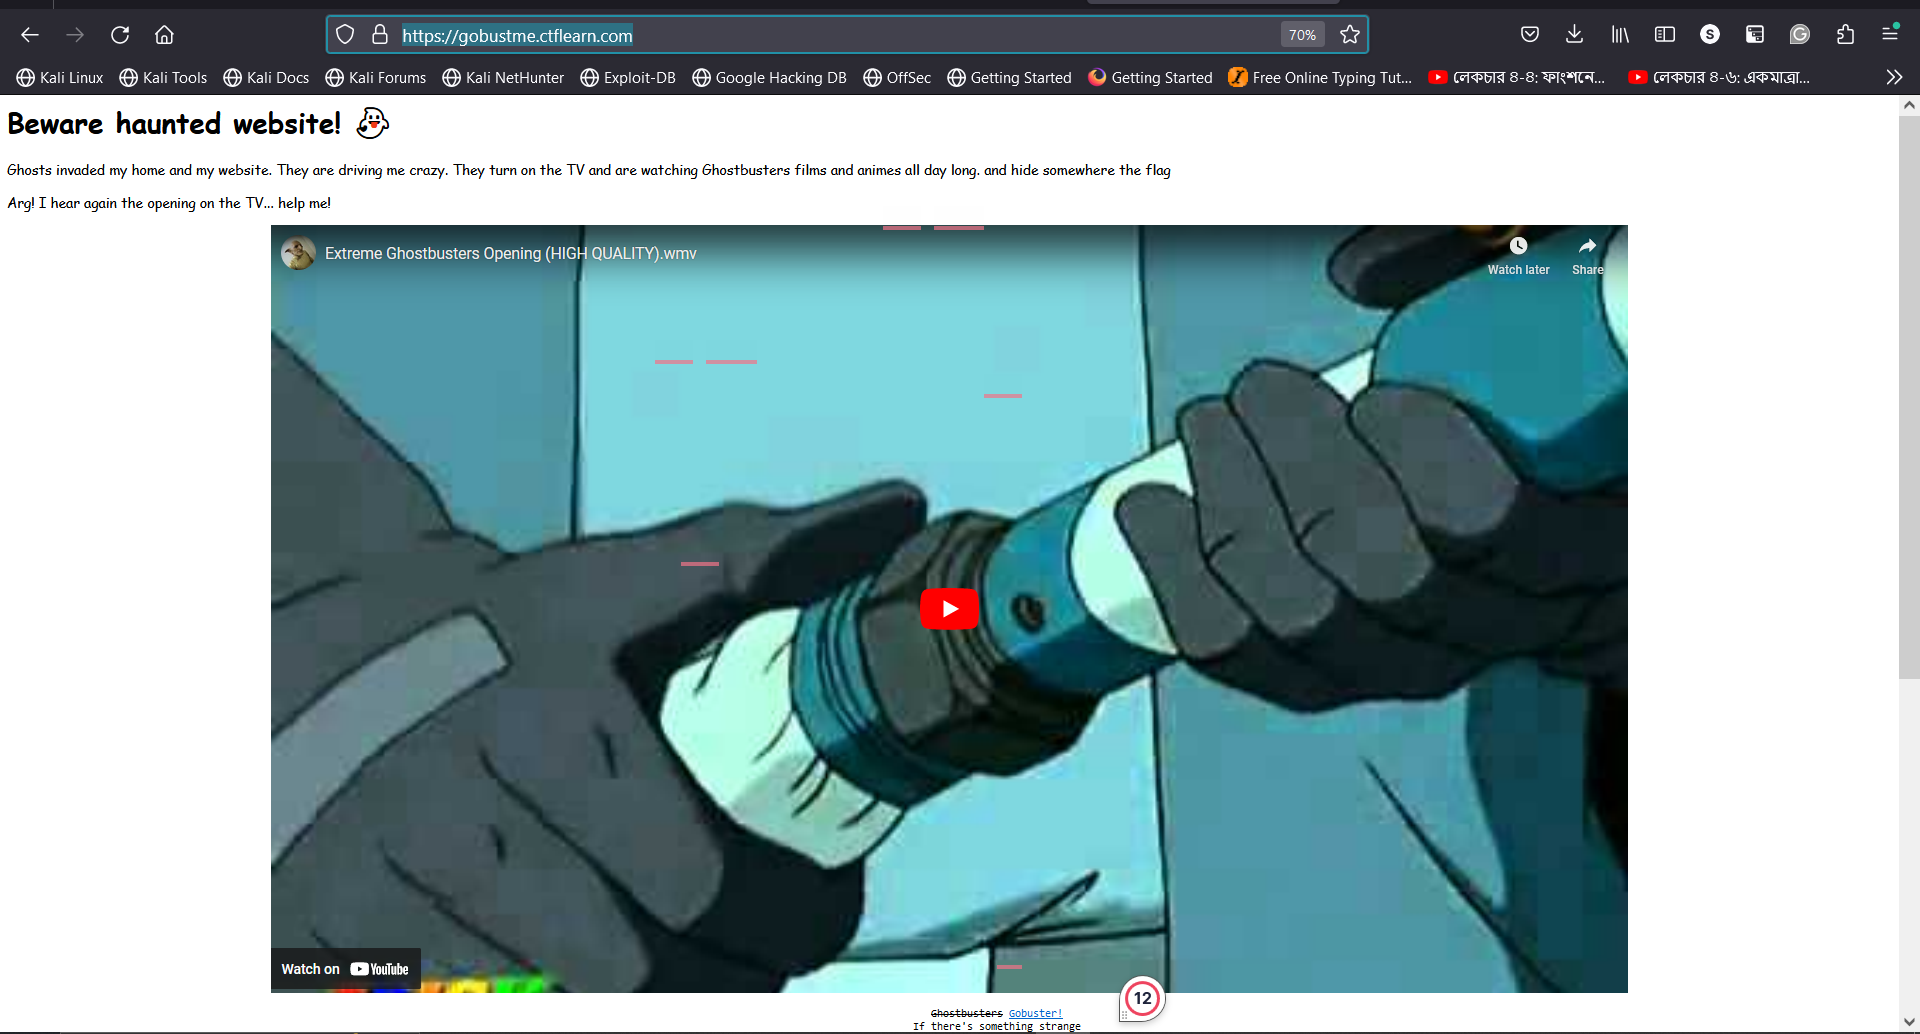
\includegraphics[width=0.5\textwidth]{dir_5.png}
    \caption{Problem Statement of gobustme}
    \label{fig: dir5 Output}
\end{figure}
For solving the problem we scan the website using directory busting.
The given Command:
\begin{lstlisting}
    gobuster dir -u https://gobustme.ctflearn.com -w common1.txt 
\end{lstlisting}
The output for this is as follows:
\begin{figure}[H]
    \centering
    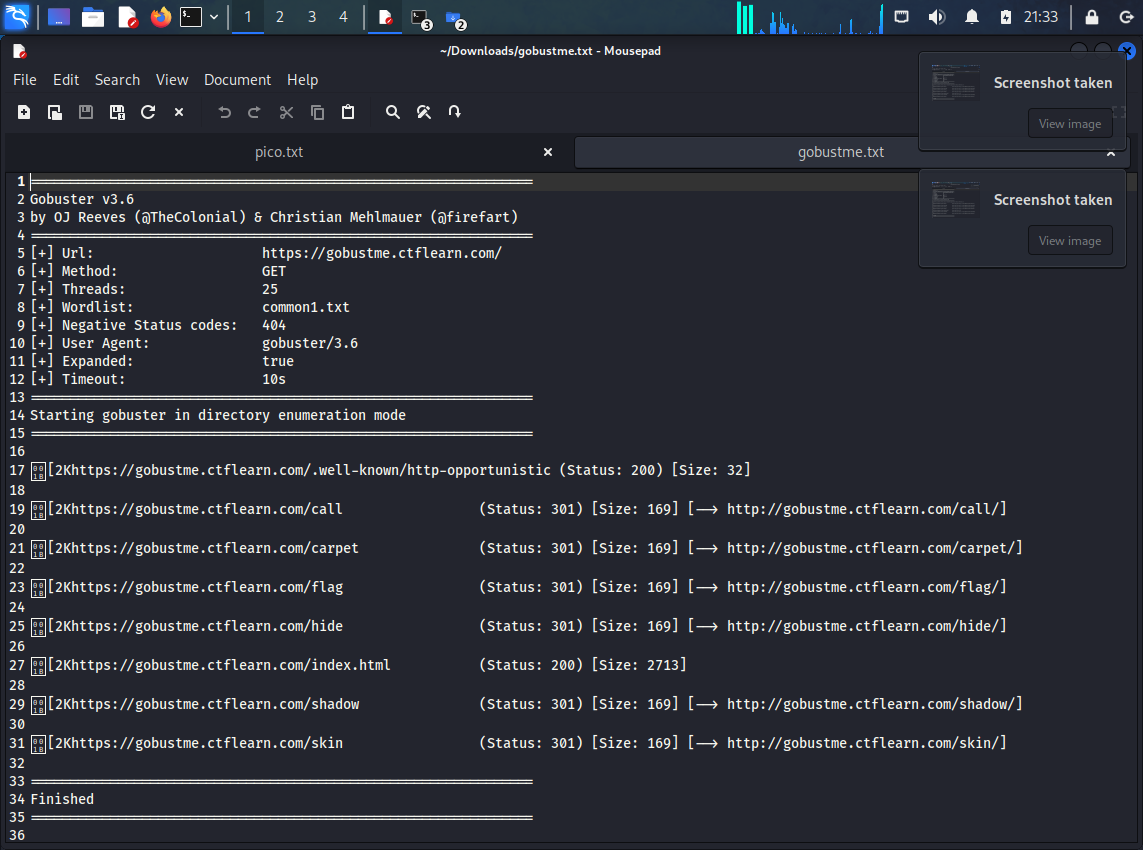
\includegraphics[width=0.6\textwidth]{dir_6.png}
    \caption{output of scanning gobustme}
    \label{fig: dir6 Output}
\end{figure}
We can access \href{https://gobustme.ctflearn.com/hide/}{Flag hidden Site} and get the flag. \\ \\
The flag: CTFlearn{gh0sbu5t3rs_4ever}
\subsection{DNS}
By dns busting, we can discover the subdomains of a site. We can again take cse.buet.ac.bd as example. \\
\textbf{\underline{The command for the discovery:}}
\begin{lstlisting}
$ gobuster dns -d cse.buet.ac.bd -w subdomains-top1million-5000.txt -t 25 
\end{lstlisting}
\textbf{\underline{The discovery:}}
\begin{lstlisting}
===============================================================
Gobuster v3.6
by OJ Reeves (@TheColonial) & Christian Mehlmauer (@firefart)
===============================================================
[+] Domain:     cse.buet.ac.bd
[+] Threads:    25
[+] Timeout:    1s
[+] Wordlist:   subdomains-top1million-5000.txt
===============================================================
Starting gobuster in DNS enumeration mode
===============================================================

[2KFound: moodle.cse.buet.ac.bd

[2KFound: ra.cse.buet.ac.bd

===============================================================
Finished
===============================================================
\end{lstlisting}
We have found 2 subdomains of cse.buet.ac.bd. One is moodle and another is ra.
\subsection{VHOST}
Now using vhost mode we will try to access the subsdomains. \\
\textbf{\underline{The Command: }}\\
\begin{lstlisting}
$ gobuster vhost -u  google.com -w subdomains-top1million-5000.txt -t 25 --append-domain    
\end{lstlisting}
\textbf{\underline{The Output:}}
\begin{figure}[H]
    \centering
    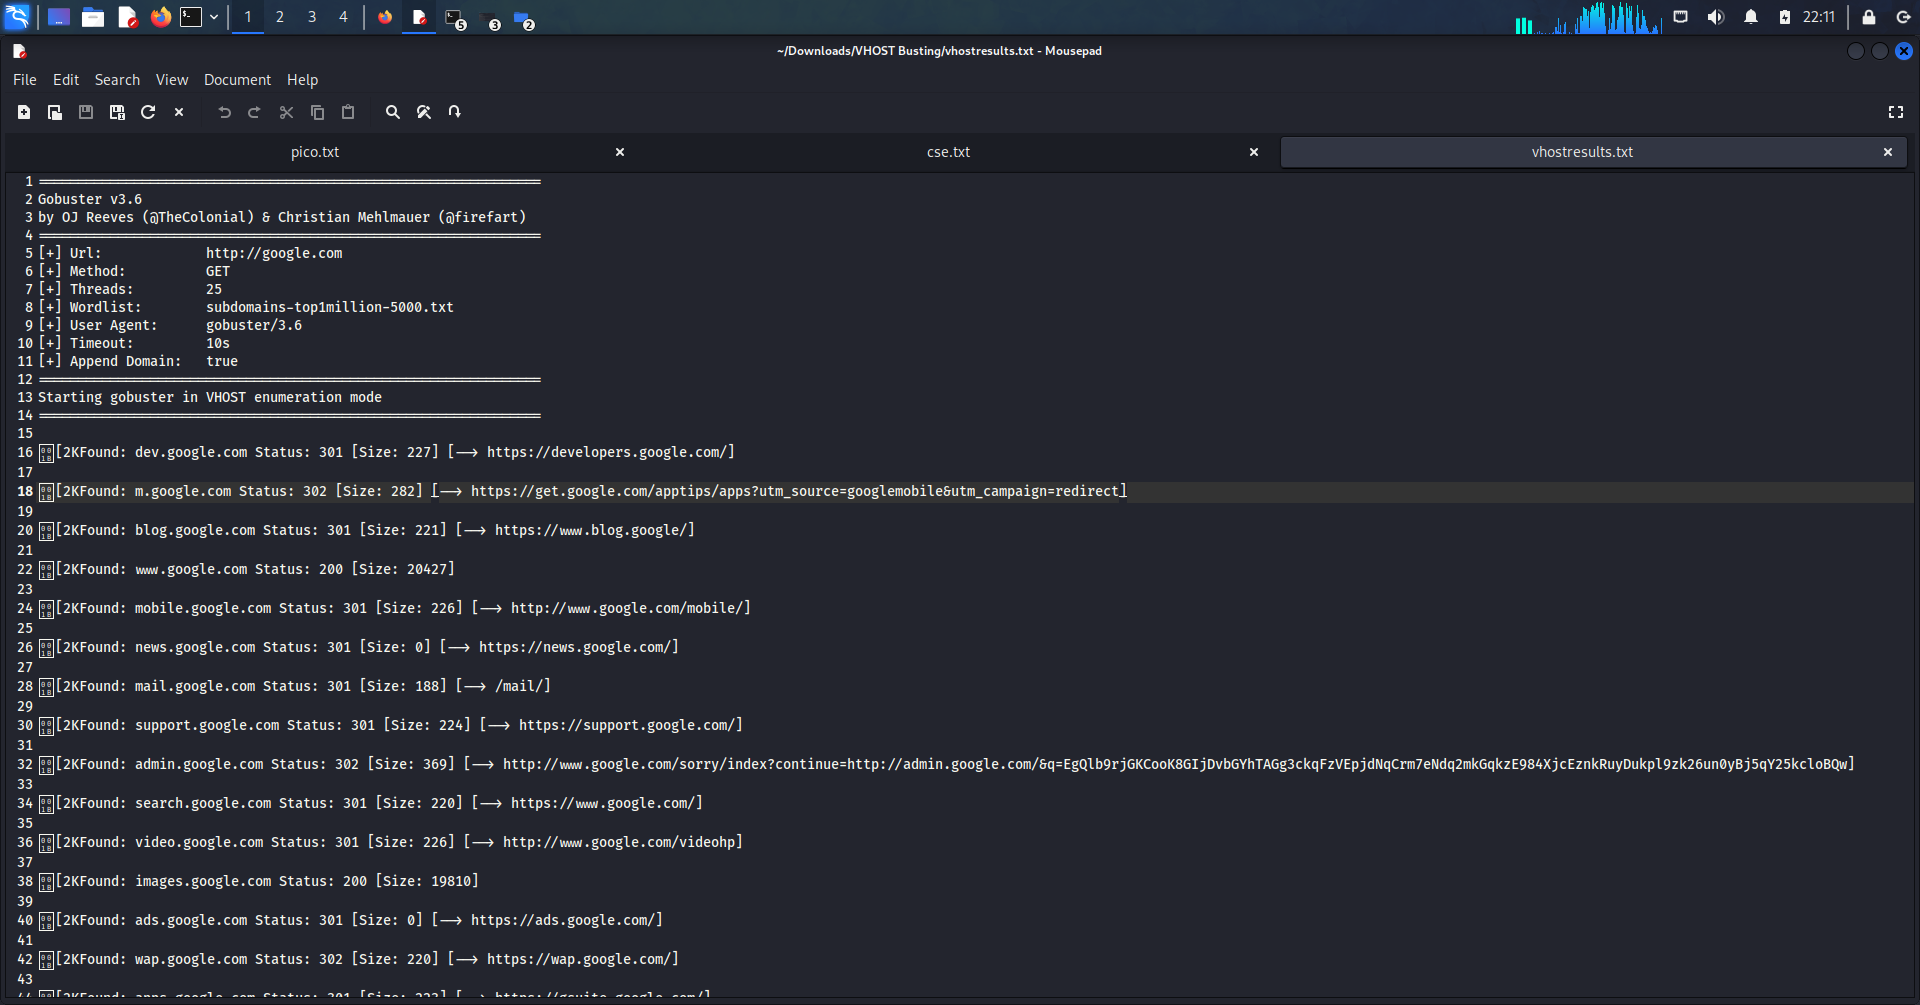
\includegraphics[width=0.7\textwidth]{1.png}
    \caption{Output of the vhost mode on google.com}
    \label{fig: vhost Output}
\end{figure}
\subsection{FUZZ}
In this mode, we replace the word \textbf{FUZZ} by a word of the word file each time and find valid parameters for the url. We are using a word file from Seclists from this link\cite{seclists} For demonstration, we are using the following command:
\begin{lstlisting}[language=bash]
gobuster fuzz -u https://play.picoctf.org/practice?FUZZ=1 -w /home/piyal/SecLists/Discovery/Web-Content/BurpSuite-ParamMiner/lowercase-headers -b 400,301 > fuzz2.txt
\end{lstlisting}
Different parts of the command are explained below:
\begin{itemize}
    \item fuzz: fuzz mode of operation
    \item -u: The target url, with the word \textbf{FUZZ}, that will be replaced by a word from the word file 
    \item -w: Path to the wordlist file
    \item -b: The status code 400 and 301 are blocked, so we will not get any response with status code 400 or 301
    \item: fuzz2.txt: The output will be written to fuzz2.txt file
\end{itemize}
The output is shown below:
\begin{figure}[H]
    \centering
    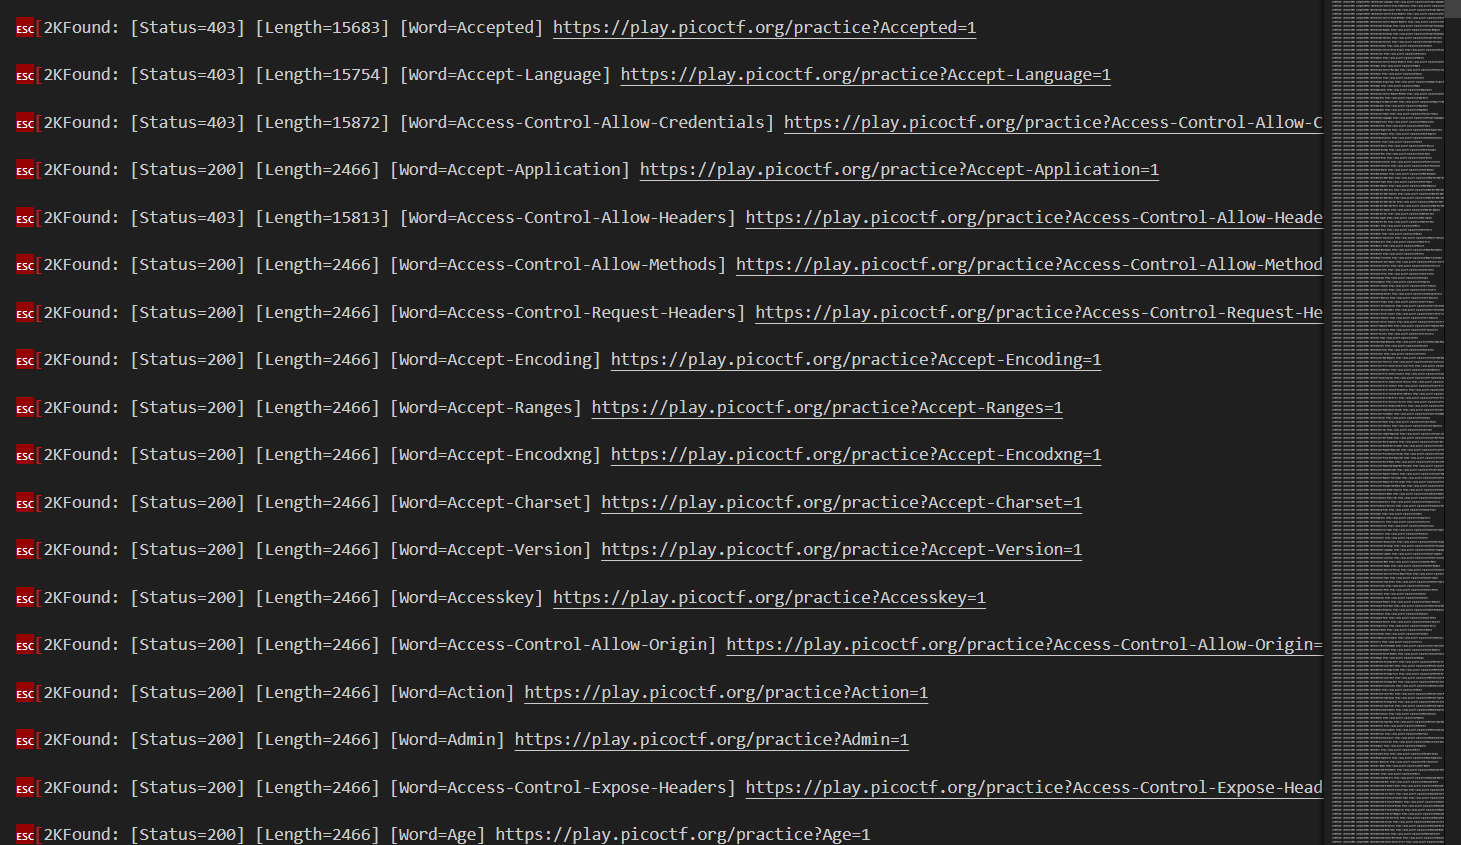
\includegraphics[width=0.5\textwidth]{Fuzz_Output.png}
    \caption{Output of the fuzz mode}
    \label{fig: FUZZ Output}
\end{figure}
\newline
We can select a link from the file and view the contents of the link:\\
\begin{figure}[H]
    \centering
    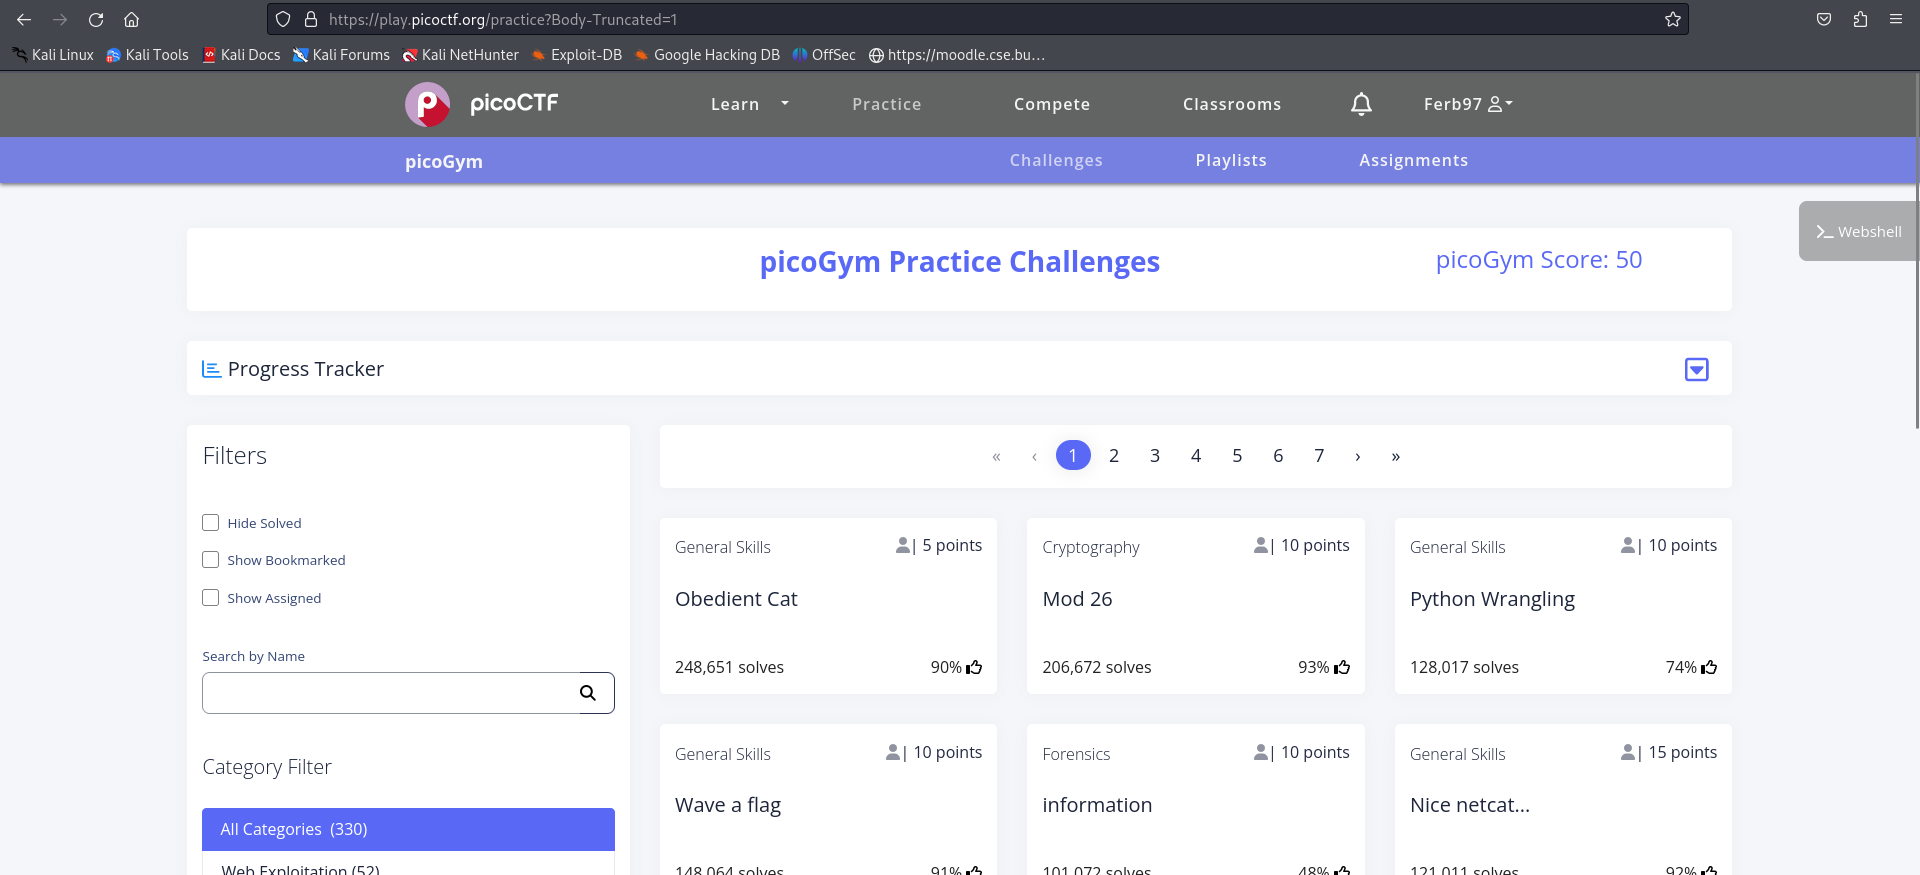
\includegraphics[width=0.5\textwidth]{Fuzz_Output_Link.png}
    \caption{Output result of the fuzz mode}
    \label{fig: FUZZ Output Result}
\end{figure}
\newline
Here, the \textbf{FUZZ} got replaced by the word \textbf{truncated}, and we can see the results. This means \textbf{truncated} is a valid parameter to the website. The attackers can use this mode to find valid parameters to launch attacks by injecting values in the parameters.

\subsection{GCS}
GCS mode finds the publicly available buckets from google cloud storage for a given word file. For demonstration, we are using the text file \textbf{s3words.txt}. We run the following command:
\begin{lstlisting}[language=bash]
gobuster gcs -w s3words.txt -t 10 > gcs1.txt 
\end{lstlisting}
Different parts of the command are explained below:
\begin{itemize}
    \item gcs: gcs mode of operation
    \item -w: Path to the wordlist file
    \item -t: number of threads
    \item: gcs1.txt: The output will be written to gcs1.txt file
\end{itemize}
The output is shown below:
\begin{figure}[H]
    \centering
    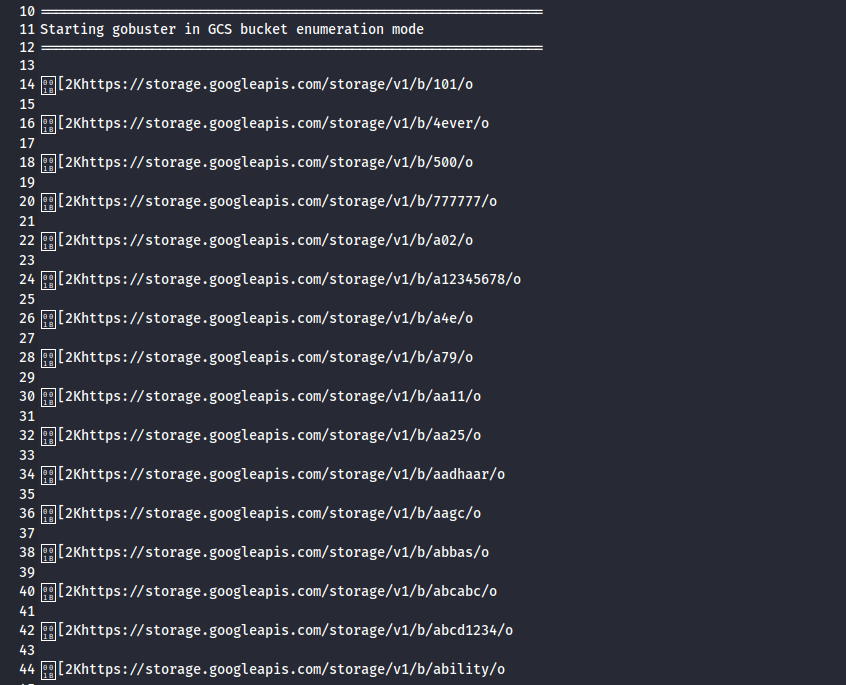
\includegraphics[width=0.5\textwidth]{gcs_Output.png}
    \caption{Output of the gcs mode}
    \label{fig: gcs Output}
\end{figure}
\newline
If we paste this link, we will get an output like the following:
\begin{figure}[H]
    \centering
    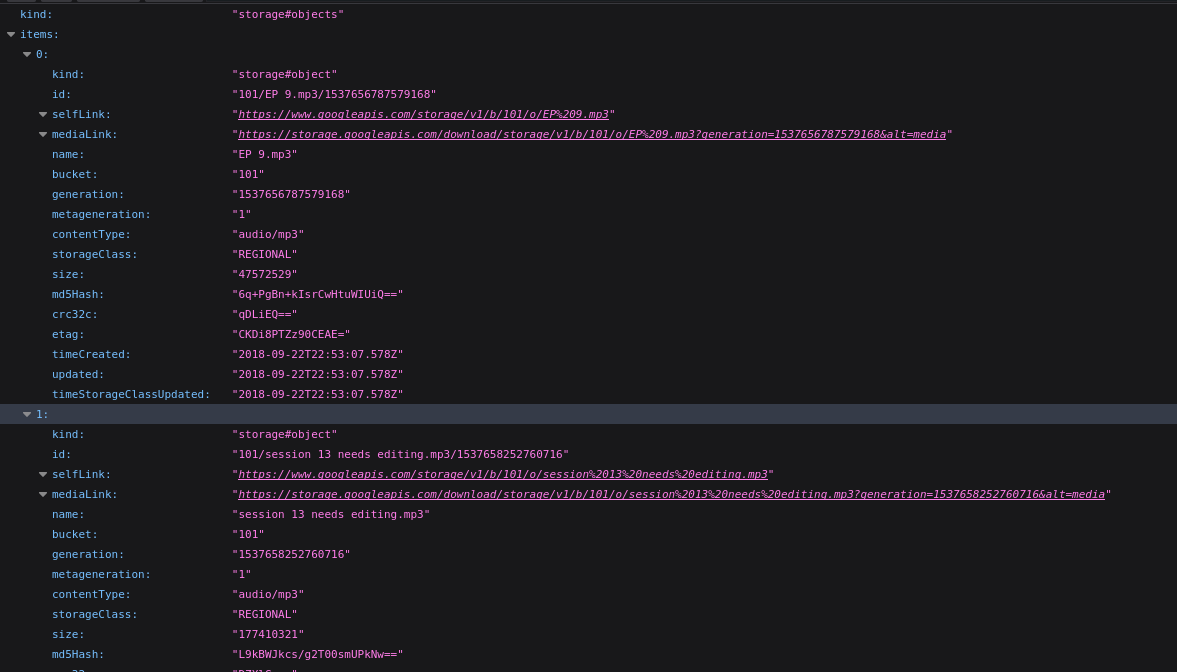
\includegraphics[width=0.5\textwidth]{gcs_Output_MediaLink.png}
    \caption{Output Media Link of the gcs mode}
    \label{fig: gcs Output Media Link}
\end{figure}
\newline
The \textbf{mediaLink} part contains the link for the file. All files are not accessible here. So, if we want to access the links, we may get a status 403 code.
\begin{figure}[H]
    \centering
    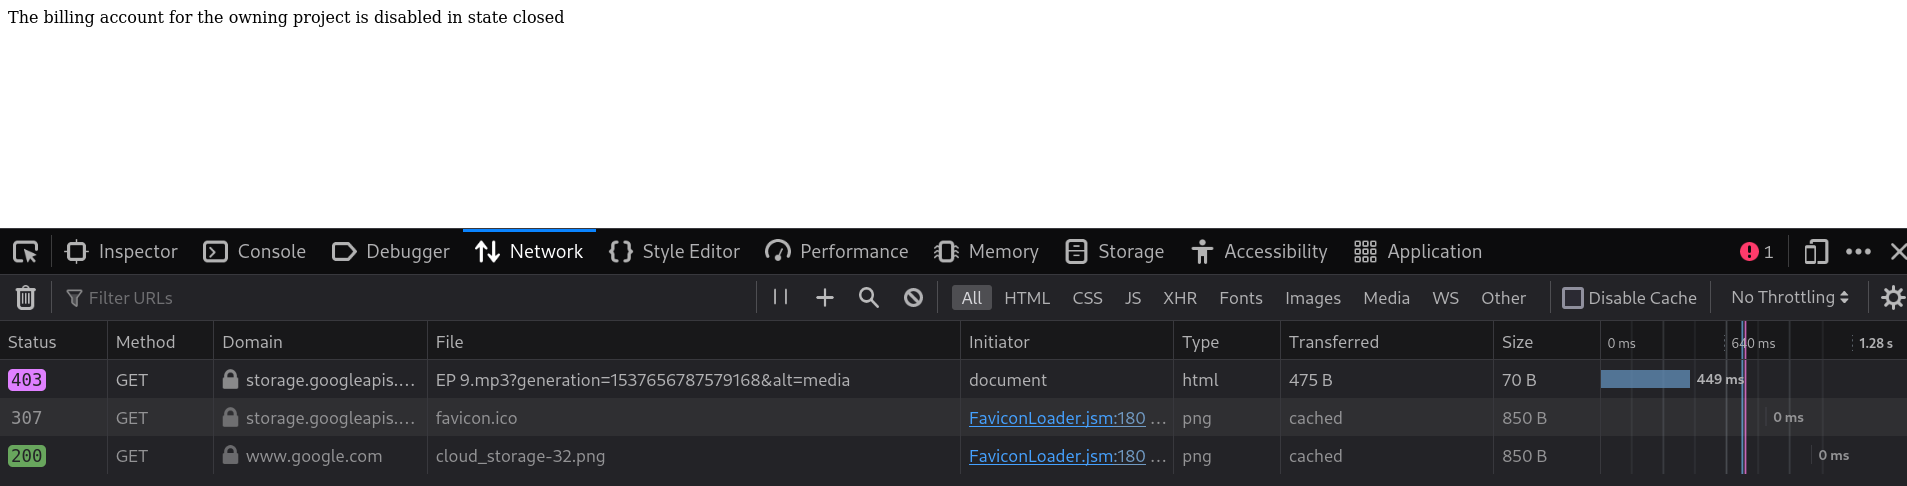
\includegraphics[width=0.5\textwidth]{gcs_Output_Fail.png}
    \caption{Failed Output of the gcs mode}
    \label{fig: gcs Output Fail}
\end{figure}
To find out which links are accessible, we write a python file named \textbf{find\_working\_links.py}. The function of the python file is explained below:
\begin{itemize}
    \item It reads the output from \textbf{gcs1.txt} file.
    \item Then it formats the so they can be used to find files.
    \item The formatted links are then written to \textbf{formatted\_links.txt} file.
    \item Now, we read the \textbf{formatted\_links.txt} file and send request.
    \item If the status code of the response is 200, we extract the \textbf{mediaLink} part and send request to know if the media exists.
    \item If we get a status response 200, we write the \textbf{link}, \textbf{mediaLink} and \textbf{File type} to \textbf{working\_links.txt} file.
    \item Thus we get all the working media links in \textbf{working\_links.txt} file.
\end{itemize}
\begin{figure}[H]
    \centering
    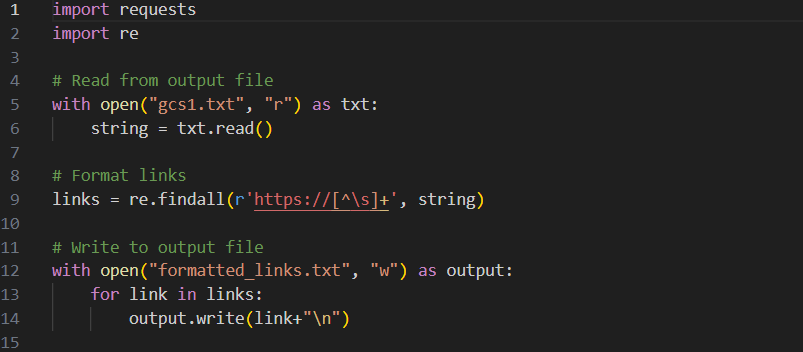
\includegraphics[width=0.5\textwidth]{gcs_Output_Formatting_Code.png}
    \caption{Code for formatting the gcs output}
    \label{fig: gcs Output Formatting Code}
\end{figure}

\begin{figure}[H]
    \centering
    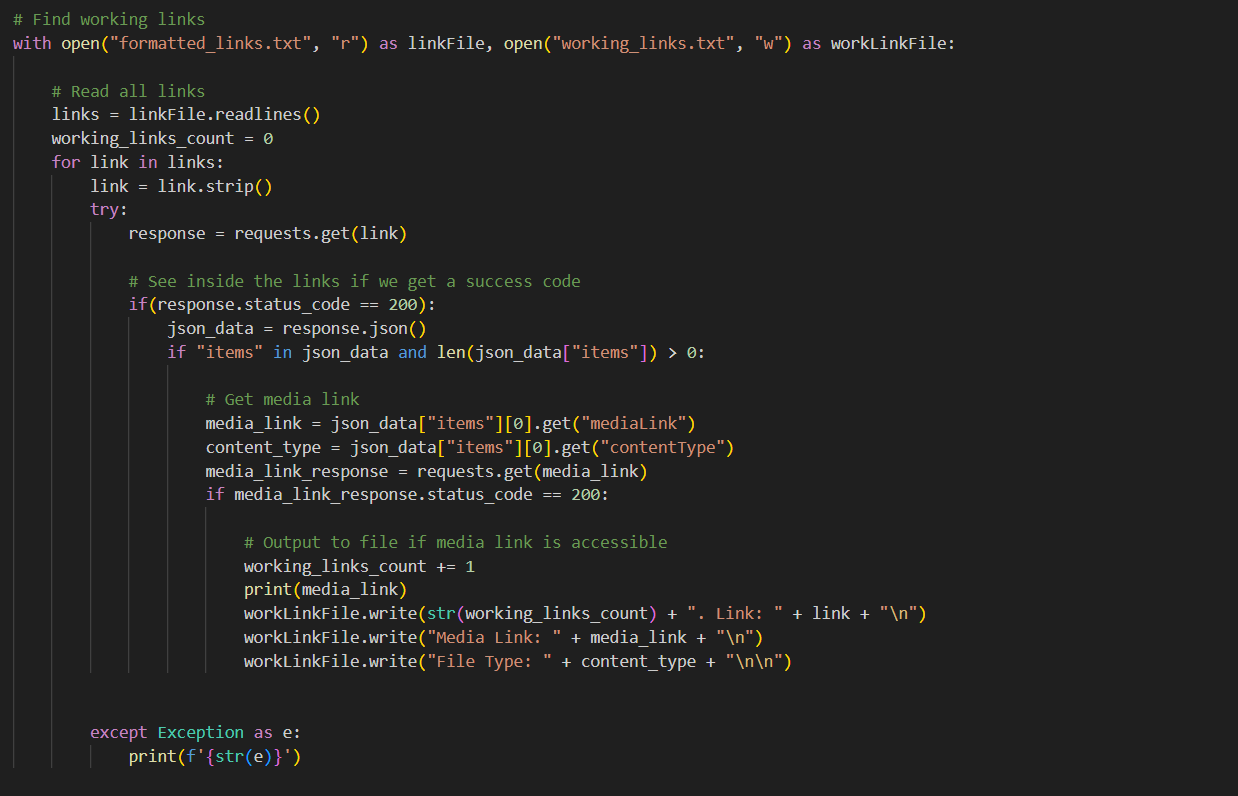
\includegraphics[width=0.5\textwidth]{gcs_Success_Links_Finding_Code.png}
    \caption{Code for finding available medias from the formatted gcs output}
    \label{fig: gcs Success Links Finding Code}
\end{figure}
The formatted links and found available media links are given below from the output files.
\begin{figure}[H]
    \centering
    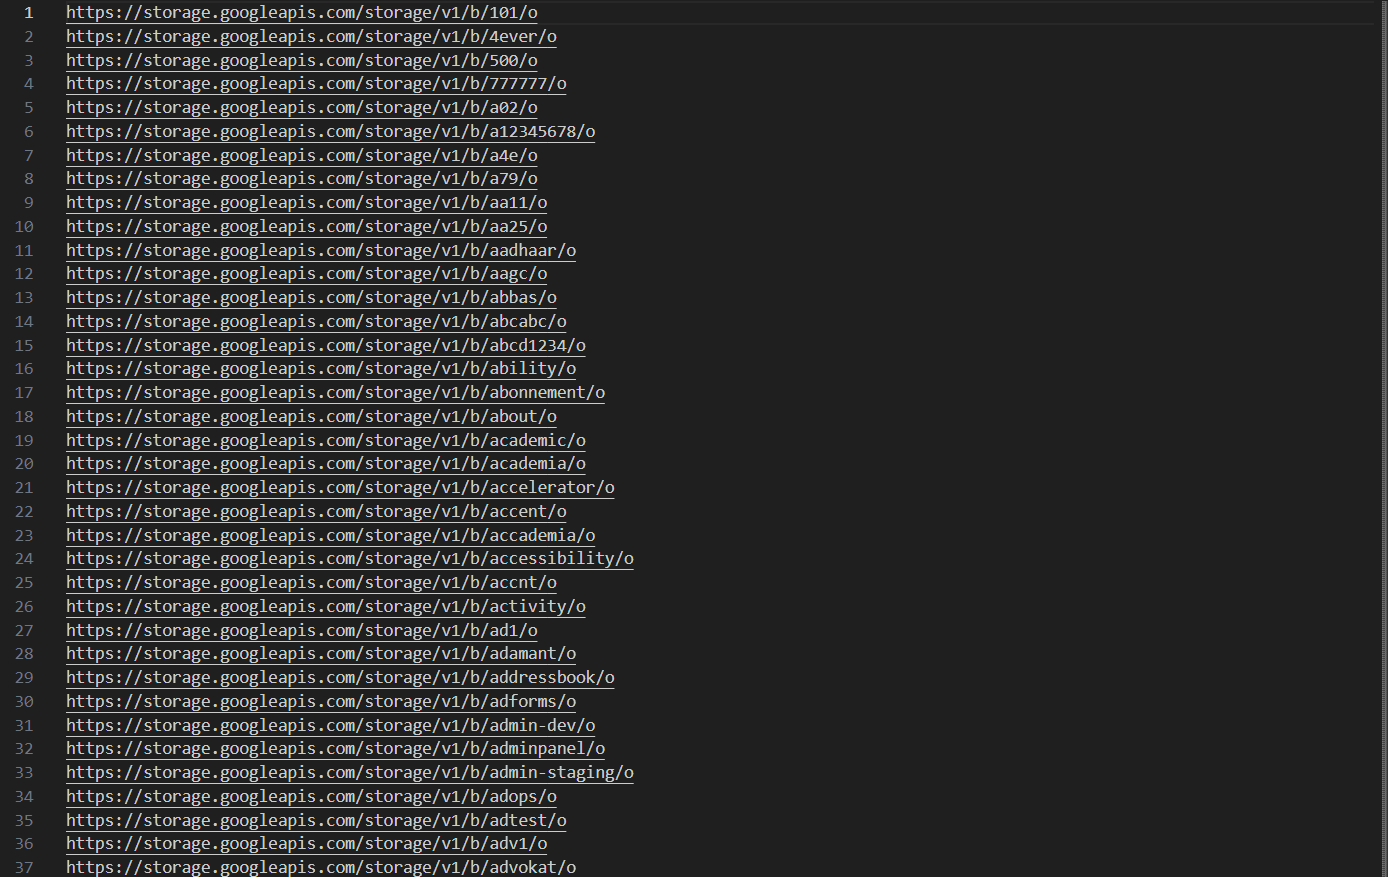
\includegraphics[width=0.5\textwidth]{gcs_Output_Formatted_Links.png}
    \caption{Links after formatting the gcs output}
    \label{fig: gcs Output Formatted Links}
\end{figure}

\begin{figure}[H]
    \centering
    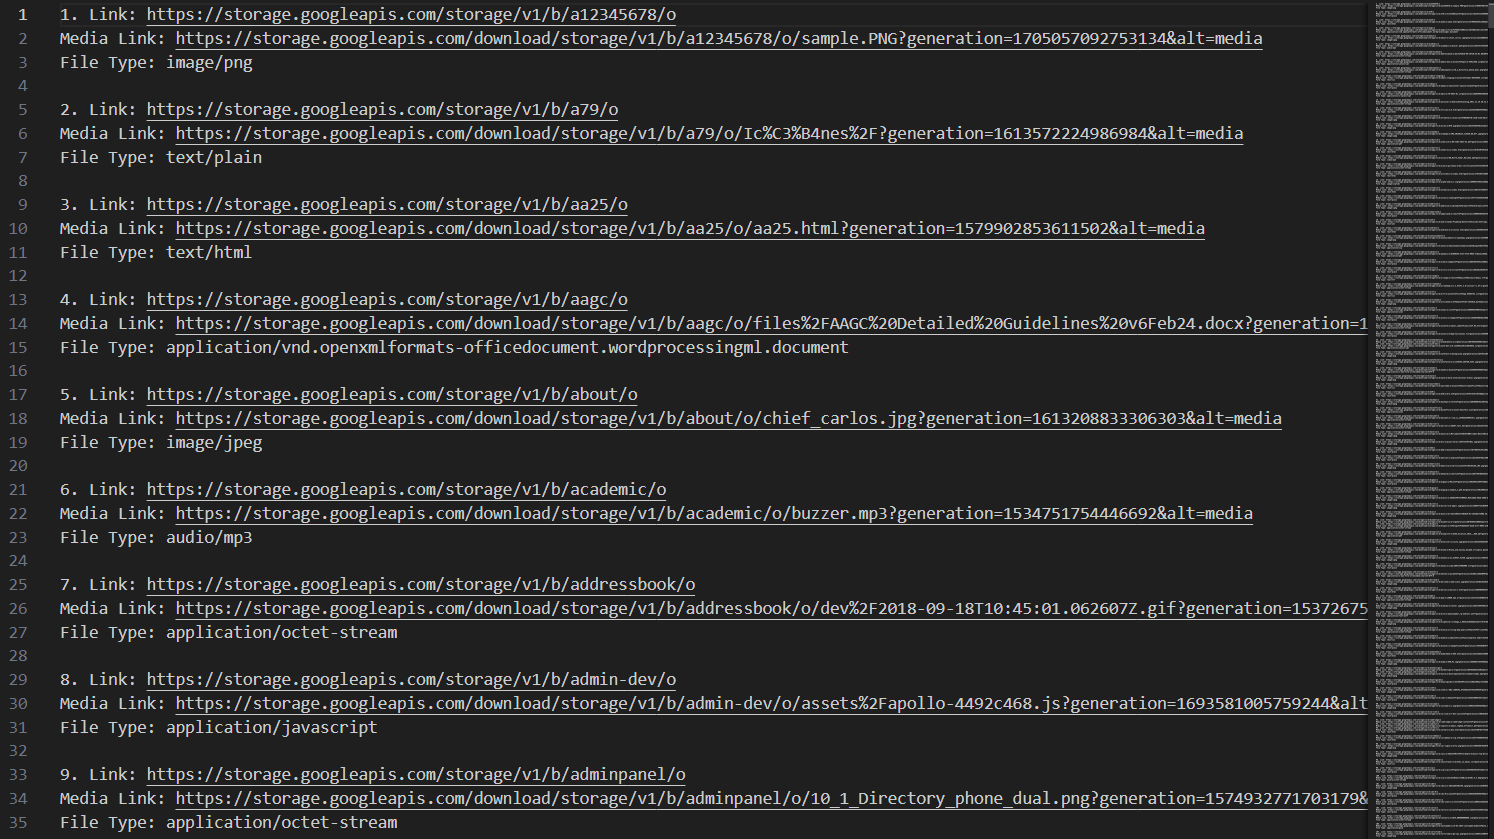
\includegraphics[width=0.5\textwidth]{gcs_Success_Links.png}
    \caption{Available medias from the formatted gcs output}
    \label{fig: gcs Success Links}
\end{figure}
If we paste the available media links, we can find the available media files. The \textbf{output files}, python code and necessary files are given in the following github link: \cite{github_output}
\begin{figure}[H]
    \centering
    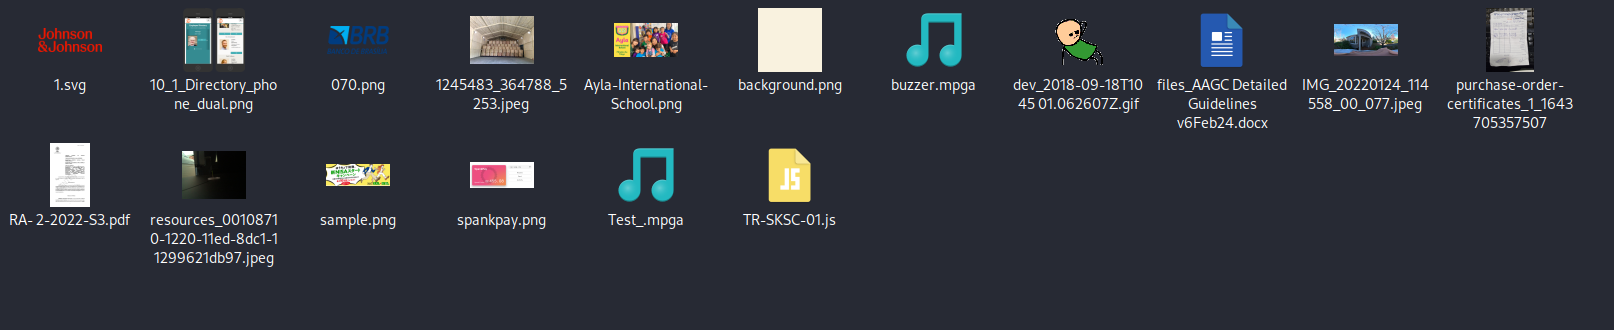
\includegraphics[width=0.5\textwidth]{gcs_Output_Files.png}
    \caption{Available medias files from the gcs output}
    \label{fig: gcs Output Files}
\end{figure}


\subsection{S3}
In this mode, gobuster looks up for the words in the word files for amazon s3 buckets. Here, we have used a modified file, named \textbf{s3wordsv1.txt} The command for this mode is given below:
\begin{lstlisting}[language=bash]
gobuster s3 -w s3wordsv1.txt -t 10 > s34.txt
\end{lstlisting}
Different parts of the command are explained below:
\begin{itemize}
    \item s3: s3 mode of operation
    \item -w: Path to the wordlist file
    \item -t: number of threads
    \item: s34.txt: The output will be written to s34.txt file
\end{itemize}
The output for this command is given below:
\begin{figure}[H]
    \centering
    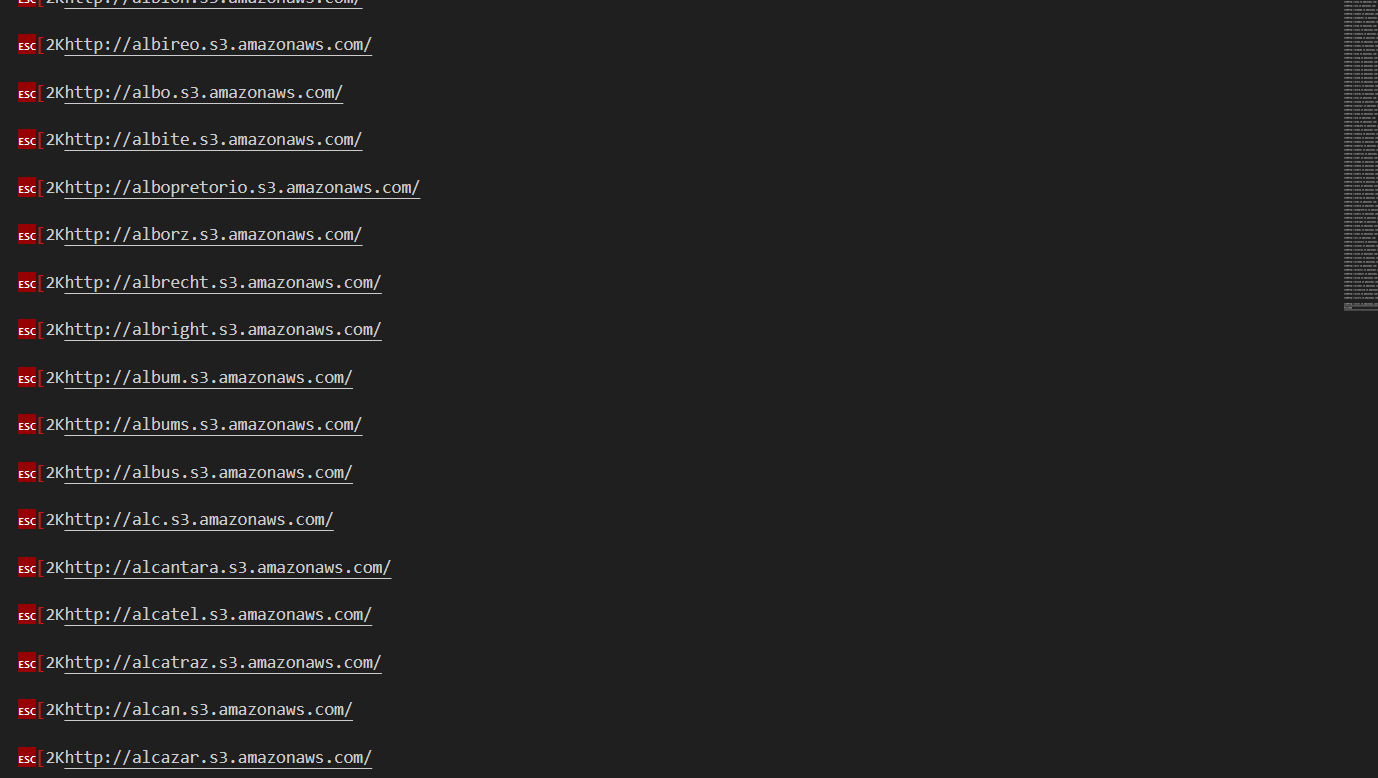
\includegraphics[width=0.5\textwidth]{s3_Output.png}
    \caption{Output of the s3 mode}
    \label{fig: s3 Output}
\end{figure}
\newline
Most of the links are not accessible. They show the code \textbf{AccessDenied}.
\begin{figure}[H]
    \centering
    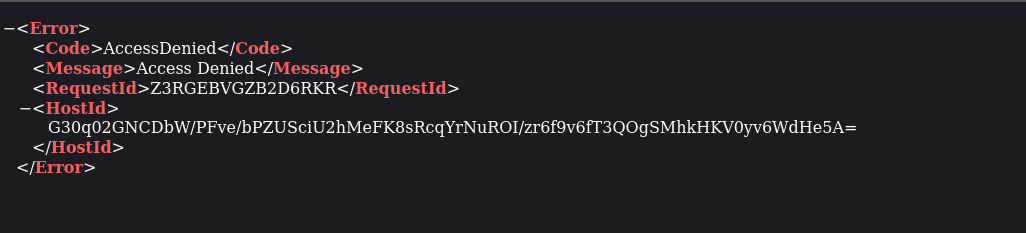
\includegraphics[width=0.5\textwidth]{s3_Output_Fail.png}
    \caption{Output Access Denied the s3 mode}
    \label{fig: s3 Output Access Denied}
\end{figure}
\newline
We found a link that gives us two links.
\begin{figure}[H]
    \centering
    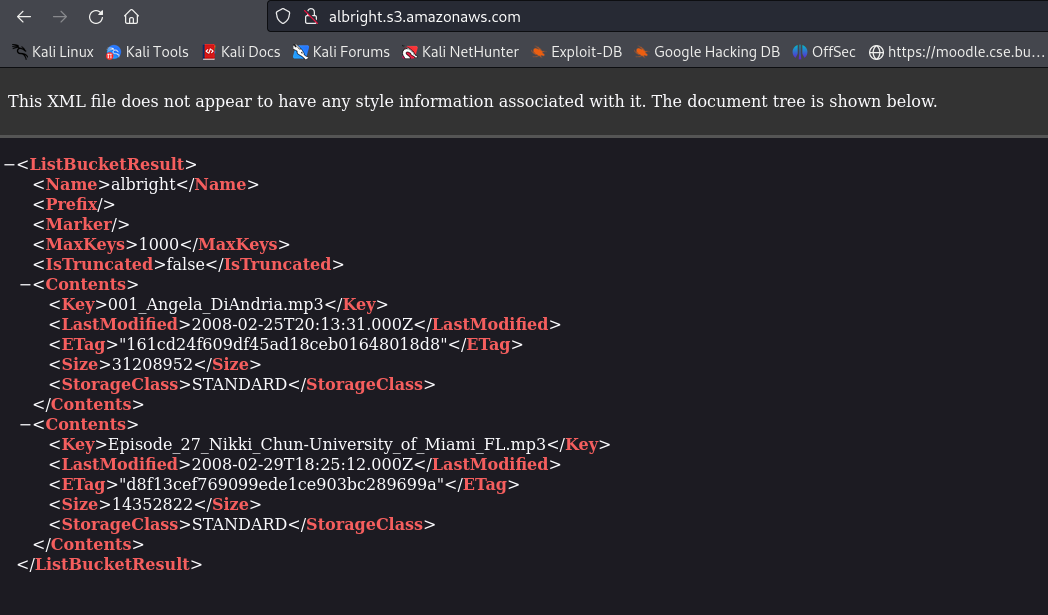
\includegraphics[width=0.5\textwidth]{s3_Output_Success.png}
    \caption{Output Success for the s3 mode}
    \label{fig: s3 Output Success}
\end{figure}
\newline
We can view the files by putting the file name after the link separated by a slash. Thus we can get publicly available amazon s3 bucket files.
\begin{figure}[H]
    \centering
    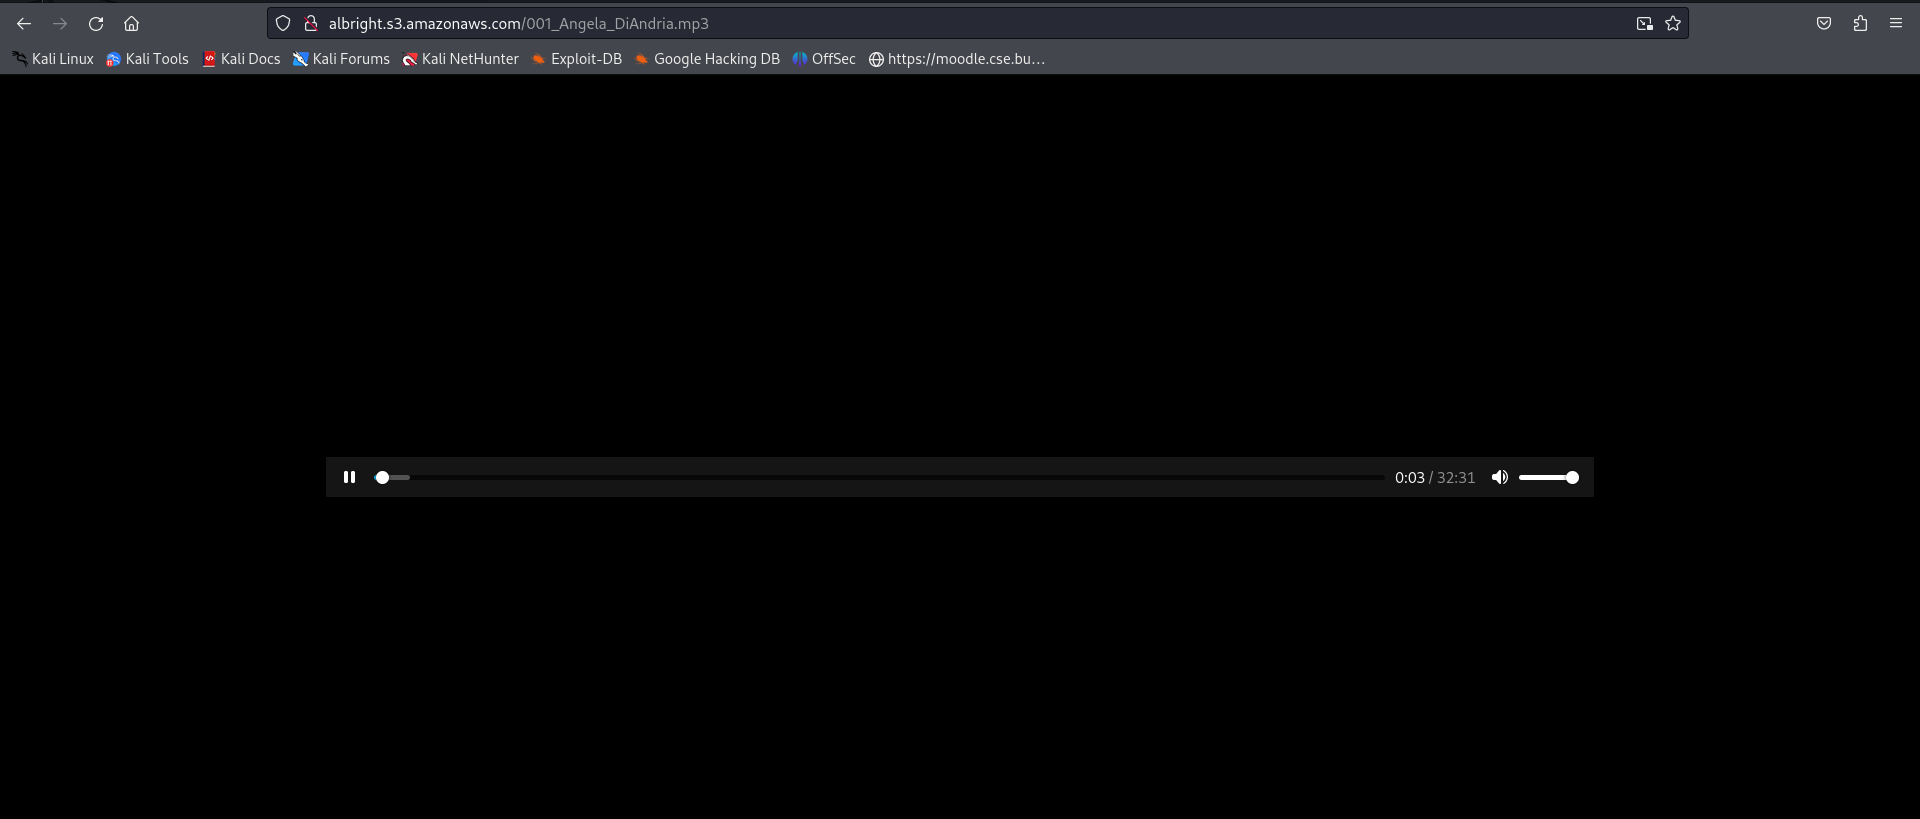
\includegraphics[width=0.5\textwidth]{s3_Output_Success_File.png}
    \caption{Output File for the s3 mode}
    \label{fig: s3 Output Success File}
\end{figure}
\newline
The files that we found are given in the github link \cite{github_output}.
\subsection{TFTP}
TFTP (Trivial File Transfer Protocol) is a simple file transfer protocol. It does not have any authentication protocol like ftp servers. So, it is not suitable for remote networks. Rather, it is set up in a local environment. We set up a tftp server on localhost in \textbf{ubuntu}(as we faced some problems setting it up on kali linux), following this link \cite{tftp}.\\
The tftp server was set up on the directory \textbf{/tftpboot}. It had the following files:
\begin{figure}[H]
    \centering
    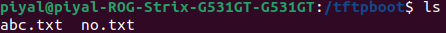
\includegraphics[width=0.5\textwidth]{tftp_Server_Files.png}
    \caption{Files in the tftp server}
    \label{fig: tftp Server Files}
\end{figure}
Then we used gobuster to enumerate over the files and find any file mentioned in the \textbf{tftpwords.txt} file. The contents of the word file is given below:
\begin{figure}[H]
    \centering
    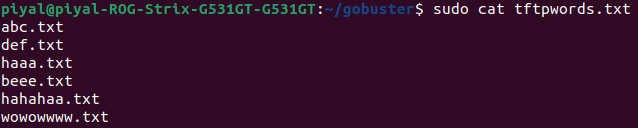
\includegraphics[width=0.5\textwidth]{tftp_Word_File.png}
    \caption{Word File for the tftp mode}
    \label{fig: tftp Word File}
\end{figure}
The command for this operation is given below:
\begin{lstlisting}[language=bash]
./gobuster tftp -s 127.0.0.1 -w tftpwords.txt
\end{lstlisting}
Different parts of the command are explained below:
\begin{itemize}
    \item tftp: tftp mode of operation
    \item -w: Path to the wordlist file
    \item -s: Link to the tftp server
\end{itemize}
As we had to set up gobuster on ubuntu for this mode and ubuntu does not support the latest gobuster version, so we built an executable file to run gobuster from the github code. For this reason, we need to run the executable file each time using \textbf{./gobuster}. As the word file contains abc.txt, we found the abc.txt file. But no.txt file was not found as it was not in the word file. Thus, we can find files on our tftp server using gobuster.
\begin{figure}[H]
    \centering
    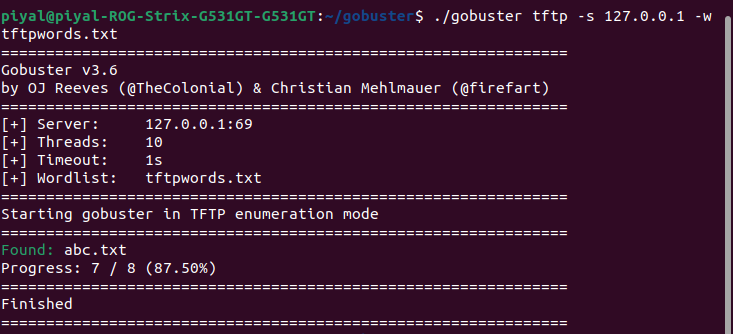
\includegraphics[width=0.5\textwidth]{tftp_Output.png}
    \caption{Output for the tftp mode}
    \label{fig: tftp Output}
\end{figure}
\printbibliography[title={References}]
\end{document}
